% =====================================================================
% BMED365 (Spring 2027) — Lab 4: Kiwi Fruit 3D Seed Segmentation Challenge
% Printable Notebook Export: 07-kiwi-neurosymbolic-ai.ipynb
% Compile with: pdflatex 07-kiwi-neurosymbolic-ai_ipynb.tex (run twice)
% =====================================================================
\documentclass[10pt,a4paper]{article}

\usepackage[utf8]{inputenc}
\usepackage[T1]{fontenc}
\usepackage[english]{babel}
\usepackage{lmodern}
\usepackage{microtype}
\usepackage{graphicx}
\usepackage{booktabs}
\usepackage{xltabular}
\usepackage{tabularx}
\usepackage{array}
\usepackage[table]{xcolor}
\usepackage{amsmath,amssymb}
\usepackage{enumitem}
\usepackage[margin=1.7cm,top=1.75cm,bottom=1.85cm,headheight=14pt]{geometry}
\usepackage{fancyhdr}
\usepackage{lastpage}
\usepackage{titlesec}
\usepackage[most]{tcolorbox}
\usepackage{listings}
\usepackage{float}
\usepackage{caption}
\usepackage[hyphens]{url}
\usepackage{hyperref}
\def\UrlBreaks{\do\/\do-\do_\do.}

% =====================================================================
% COLORS & HYPERREF (UiB / BMED365 House Style — matching NB 00 PDF)
% =====================================================================
\definecolor{uibblue}{RGB}{0, 61, 115}
\definecolor{uibred}{RGB}{175, 28, 44}
\definecolor{kiwigreen}{RGB}{27, 138, 90}
\definecolor{amberwarn}{RGB}{165, 95, 0}
\definecolor{amberbg}{RGB}{255, 250, 240}
\definecolor{lightgray}{RGB}{246, 248, 250}
\definecolor{rowalt}{RGB}{243, 247, 252}
\definecolor{codebg}{RGB}{245, 248, 252}
\definecolor{codehdr}{RGB}{224, 234, 246}
\definecolor{outbg}{RGB}{250, 250, 250}
\definecolor{outhdr}{RGB}{236, 238, 240}
\definecolor{codekw}{RGB}{0, 75, 145}
\definecolor{codestr}{RGB}{155, 35, 45}
\definecolor{codecmt}{RGB}{90, 105, 118}

\hypersetup{
    colorlinks=true,
    linkcolor=uibblue,
    citecolor=uibblue,
    urlcolor=uibred,
    pdftitle={07-kiwi-neurosymbolic-ai.ipynb -- Deep Dive into Differentiable Neurosymbolic AI on 7T MRI (BMED365 Spring 2027)},
    pdfauthor={Arvid Lundervold (UiB / MMIV) -- BMED365 Spring 2027}
}

% =====================================================================
% TYPOGRAPHY, HEADERS & CALLOUT BOXES
% =====================================================================
\setlength{\parindent}{0pt}
\setlength{\parskip}{0.42em}
\setlist[itemize]{topsep=2pt,itemsep=2pt,leftmargin=1.4em}
\setlist[enumerate]{topsep=2pt,itemsep=2pt,leftmargin=1.6em}

\newcolumntype{L}[1]{>{\raggedright\arraybackslash}p{#1}}
\newcolumntype{C}[1]{>{\centering\arraybackslash}p{#1}}
\newcolumntype{R}[1]{>{\raggedleft\arraybackslash}p{#1}}
\newcolumntype{Y}{>{\raggedright\arraybackslash}X}

\titleformat{\section}{\large\bfseries\color{uibblue}}{\thesection}{0.65em}{}[\vspace{1pt}\color{uibblue!40}\titlerule]
\titleformat{\subsection}{\normalsize\bfseries\color{uibblue!88!black}}{\thesubsection}{0.55em}{}
\titleformat{\subsubsection}{\small\bfseries\color{uibblue!75!black}}{\thesubsubsection}{0.5em}{}
\titlespacing*{\section}{0pt}{1.05em}{0.4em}
\titlespacing*{\subsection}{0pt}{0.75em}{0.25em}
\titlespacing*{\subsubsection}{0pt}{0.55em}{0.2em}

\pagestyle{fancy}
\fancyhf{}
\fancyhead[L]{\footnotesize\textcolor{gray}{BMED365 (Spring 2027) $\cdot$ Lab 4: Kiwi 7T MRI Challenge}}
\fancyhead[R]{\footnotesize\textcolor{gray}{\texttt{07-kiwi-neurosymbolic-ai.ipynb}}}
\fancyfoot[L]{\footnotesize\textcolor{gray}{University of Bergen \& MMIV $\cdot$ \href{https://github.com/arvidl/BMED365-2027}{\textcolor{gray}{github.com/arvidl/BMED365-2027}}}}
\fancyfoot[R]{\footnotesize\textcolor{gray}{Page \thepage{} of \pageref{LastPage}}}
\renewcommand{\headrulewidth}{0.4pt}
\renewcommand{\footrulewidth}{0.2pt}

\fancypagestyle{firstpage}{
    \fancyhf{}
    \fancyfoot[L]{\footnotesize\textcolor{gray}{University of Bergen \& MMIV $\cdot$ \href{https://github.com/arvidl/BMED365-2027}{\textcolor{gray}{github.com/arvidl/BMED365-2027}}}}
    \fancyfoot[R]{\footnotesize\textcolor{gray}{Page \thepage{} of \pageref{LastPage}}}
    \renewcommand{\headrulewidth}{0pt}
    \renewcommand{\footrulewidth}{0.2pt}
}

% --- Notebook Cell & Pedagogical Boxes ---
\newtcolorbox{seqbox}[1][]{
    enhanced, breakable,
    colback=lightgray, colframe=uibblue,
    colbacktitle=uibblue, coltitle=white,
    fonttitle=\bfseries\small, title={#1},
    boxrule=0.6pt, arc=2.5pt, left=7pt, right=7pt, top=5pt, bottom=5pt
}

\newtcolorbox{codebox}[1][]{
    enhanced, breakable,
    colback=codebg, colframe=uibblue!35,
    colbacktitle=codehdr, coltitle=uibblue!90!black,
    fonttitle=\ttfamily\scriptsize\bfseries, title={#1},
    boxrule=0.55pt, arc=2.2pt, left=6pt, right=6pt, top=3pt, bottom=3pt,
    toptitle=2.5pt, bottomtitle=2.5pt
}

\newtcolorbox{outbox}[1][]{
    enhanced, breakable,
    colback=outbg, colframe=gray!45,
    colbacktitle=outhdr, coltitle=black!75,
    fonttitle=\ttfamily\scriptsize\bfseries, title={#1},
    boxrule=0.5pt, arc=2.2pt, left=6pt, right=6pt, top=3pt, bottom=3pt,
    toptitle=2pt, bottomtitle=2pt
}

\newtcolorbox{clinbox}[1][]{
    enhanced, breakable,
    colback=amberbg, colframe=amberwarn,
    colbacktitle=amberwarn, coltitle=white,
    fonttitle=\bfseries\small, title={#1},
    boxrule=0.6pt, arc=2.5pt, left=7pt, right=7pt, top=5pt, bottom=5pt
}

\newtcolorbox{qabox}[1][]{
    enhanced,
    colback=kiwigreen!6, colframe=kiwigreen!85!black,
    colbacktitle=kiwigreen!85!black, coltitle=white,
    fonttitle=\bfseries\small, title={#1},
    boxrule=0.6pt, arc=2.5pt, left=7pt, right=7pt, top=5pt, bottom=5pt
}

\lstdefinestyle{pybmed}{
    language=Python,
    basicstyle=\ttfamily\scriptsize,
    keywordstyle=\bfseries\color{codekw},
    stringstyle=\color{codestr},
    commentstyle=\itshape\color{codecmt},
    showstringspaces=false,
    breaklines=true,
    breakatwhitespace=true,
    breakindent=12pt,
    columns=fullflexible,
    keepspaces=true,
    upquote=true,
    aboveskip=2pt,
    belowskip=2pt,
    xleftmargin=0pt,
    xrightmargin=0pt
}

\lstdefinestyle{outbmed}{
    basicstyle=\ttfamily\scriptsize\color{black!85},
    showstringspaces=false,
    breaklines=true,
    breakatwhitespace=false,
    columns=fullflexible,
    keepspaces=true,
    upquote=true,
    aboveskip=1pt,
    belowskip=1pt,
    xleftmargin=0pt,
    xrightmargin=0pt
}

\newcommand{\ghblob}{https://github.com/arvidl/BMED365-2027/blob/main}
\newcommand{\colabbase}{https://colab.research.google.com/github/arvidl/BMED365-2027/blob/main}
\newcommand{\colabbtn}[1]{%
  \href{#1}{\tcbox[on line, arc=2.5pt, boxsep=0pt, left=6pt, right=6pt, top=2.5pt, bottom=2.5pt,
    colback=amberwarn!85!yellow, colframe=white!70!amberwarn, boxrule=0.5pt]{%
    \sffamily\bfseries\scriptsize\color{white}Open in Google Colab}}%
}

% =====================================================================
\begin{document}
\thispagestyle{firstpage}

% --- TITLE BANNER ---
\begin{tcolorbox}[
    enhanced, colback=uibblue, colframe=uibblue,
    arc=3.5pt, left=12pt, right=12pt, top=9pt, bottom=9pt
]
{\Large\bfseries\color{white} Deep Dive into Differentiable Neurosymbolic AI on 7\,T MRI:\\
{\large Teaching Neural Networks Anatomy, MRI Physics \& Steric Geometry}}\\[4pt]
{\normalsize\color{white!90} BMED365 --- Computational Imaging, Modeling and AI in Biomedicine (Spring 2027)}\\[3pt]
{\footnotesize\color{white!82}
Arvid Lundervold (University of Bergen \& MMIV) $\;\cdot\;$
Runs locally with \texttt{uv} (\texttt{bmed365-2027} kernel) or in Google Colab (100\% pure PyTorch)
}\\[6pt]
\colabbtn{\colabbase/Lab4-Comp-Imag/Kiwi-challenge/notebooks/07-kiwi-neurosymbolic-ai.ipynb}\hspace{8pt}
{\footnotesize\href{\ghblob/Lab4-Comp-Imag/Kiwi-challenge/notebooks/07-kiwi-neurosymbolic-ai.ipynb}{\textcolor{white}{\underline{\texttt{07-kiwi-neurosymbolic-ai.ipynb} on GitHub}}}}
\end{tcolorbox}

% --- KIWI SEQUENCE BOX ---
\begin{seqbox}[Kiwi Challenge Notebook Sequence (\texttt{Lab4-Comp-Imag/Kiwi-challenge})]
\begin{enumerate}[start=0, itemsep=1.5pt, topsep=1pt, font=\footnotesize]
    \item \href{\ghblob/Lab4-Comp-Imag/Kiwi-challenge/notebooks/00-kiwi-dicom-to-nifti.ipynb}{\texttt{00-kiwi-dicom-to-nifti.ipynb}} --- History of medical image formats (\texttt{XITE/BIFF} $\to$ \texttt{DICOM} $\to$ \texttt{NIfTI} \& \texttt{BIDS}) \& converting the 128 Bruker 7\,T DICOM slices.
    \item \href{\ghblob/Lab4-Comp-Imag/Kiwi-challenge/notebooks/01-kiwi-explore.ipynb}{\texttt{01-kiwi-explore.ipynb}} --- 3D NIfTI headers, physical voxel geometry \& affine coordinate systems.
    \item \href{\ghblob/Lab4-Comp-Imag/Kiwi-challenge/notebooks/02-kiwi-seeds-explore.ipynb}{\texttt{02-kiwi-seeds-explore.ipynb}} --- 2D single-slice filtering, thresholding, unsupervised $K$-means \& the Dagstuhl/CUHK 3D variational milestone.
    \item \href{\ghblob/Lab4-Comp-Imag/Kiwi-challenge/notebooks/03-kiwi-paradigms-and-verification.ipynb}{\texttt{03-kiwi-paradigms-and-verification.ipynb}} --- Full 3D segmentation ladder, quantitative ``lesion load'', Curated 3D Micro-GT scoring \& the \textbf{4-Panel Semi-Verifiability Dashboard}.
    \item \href{\ghblob/Lab4-Comp-Imag/Kiwi-challenge/notebooks/03b-kiwi-interactive-gt-and-interrater.ipynb}{\texttt{03b-kiwi-interactive-gt-and-interrater.ipynb}} --- Interactive 3D Jupyter-Widget delineation, personalized Ground Truth (\texttt{MyStuff/}), \textbf{Inter-Rater Variability}, \textbf{Panoptic Quality ($\text{PQ}$)} \& \textbf{STAPLE Consensus}.
    \item \href{\ghblob/Lab4-Comp-Imag/Kiwi-challenge/notebooks/04-kiwi-semantic-vs-instance.ipynb}{\texttt{04-kiwi-semantic-vs-instance.ipynb}} --- Formal definitions of \textbf{Semantic, Instance \& Panoptic} segmentation and \textbf{3D PyTorch Semantic vs.\ Instance U-Nets}.
    \item \href{\ghblob/Lab4-Comp-Imag/Kiwi-challenge/notebooks/05-kiwi-promptable-foundation-models.ipynb}{\texttt{05-kiwi-promptable-foundation-models.ipynb}} --- Live \textbf{\texttt{SAM 2.1} vs.\ \texttt{MedSAM}} foundation-model workshop + 3D slice memory (\href{\ghblob/Lab4-Comp-Imag/Kiwi-challenge/docs/promptable-foundation-models.md}{\textit{guide}} $|$ \href{\ghblob/Lab4-Comp-Imag/Kiwi-challenge/docs/promptable-foundation-models.pdf}{\textit{PDF}}).
    \item \href{\ghblob/Lab4-Comp-Imag/Kiwi-challenge/notebooks/06-kiwi-frontier-ai-paradigms.ipynb}{\texttt{06-kiwi-frontier-ai-paradigms.ipynb}} --- Frontier AI capstone: \textbf{3D SSL}, \textbf{3D U-Mamba}, \textbf{Conditional Flow-Diffusion}, \& \textbf{Differentiable Neurosymbolic AI (LTN)} (\href{\ghblob/Lab4-Comp-Imag/Kiwi-challenge/docs/frontier-ai-paradigms.md}{\textit{guide}} $|$ \href{\ghblob/Lab4-Comp-Imag/Kiwi-challenge/docs/frontier-ai-paradigms.pdf}{\textit{PDF}}).
    \item \textbf{\texttt{07-kiwi-neurosymbolic-ai.ipynb} (this notebook)} --- Opening the hood on \textbf{Differentiable Neurosymbolic AI (\texttt{LTN} + Bayes Log-Odds \texttt{Organ-GPS} + \texttt{Lab 5} Hard-Core Priors)}: prior auditing, proving the \texttt{InstanceNorm3d} coordinate trap, controlled 5-model ablations, curing calibration drift, mechanistic auditing, \& clinical medical imaging translation.
\end{enumerate}
\end{seqbox}

% =====================================================================
\section*{Introduction: Why Differentiable Neurosymbolic AI Led Notebook \texttt{06}}
% =====================================================================

In \href{\ghblob/Lab4-Comp-Imag/Kiwi-challenge/notebooks/06-kiwi-frontier-ai-paradigms.ipynb}{\textbf{Notebook \texttt{06}}} (and its companion guide \href{\ghblob/Lab4-Comp-Imag/Kiwi-challenge/docs/frontier-ai-paradigms.pdf}{\texttt{frontier-ai-paradigms.pdf}}), we benchmarked four frontier AI families head-to-head on the exact same \texttt{80 $\times$ 40 $\times$ 16} (\texttt{52}-seed) strictly held-out 3D test wedge and the intact \texttt{256 $\times$ 256 $\times$ 128} 7\,T kiwifruit MRI --- alongside our supervised \texttt{3D Multi-Task U-Net} (\texttt{NB 04}) and promptable \texttt{SAM 2.1} (\texttt{NB 05}):

{\footnotesize
\renewcommand{\arraystretch}{1.24}
\rowcolors{2}{rowalt}{white}
\begin{tabularx}{\textwidth}{L{4.95cm} C{0.9cm} C{0.9cm} C{0.95cm} C{0.95cm} C{1.75cm} Y}
\toprule
\rowcolor{uibblue!12}\textbf{Paradigm (Notebooks \texttt{04}--\texttt{06})} & \textbf{PQ} & \textbf{Dice} & \textbf{SQ} & \textbf{RQ} & \textbf{Pred (GT=52)} & \textbf{Unmasked Whole-Fruit OOD Safety} \\
\midrule
\textbf{Pillar 4: \texttt{LTN} Neurosymbolic + Split} & \textbf{0.508} & \textbf{0.717} & \textbf{0.763} & 0.667 & 35 \textit{(conserv.)} & \textbf{0 polar FP voxels (-99.7\% OOD)} \\
\textbf{Pillar 3: Conditional Flow-Diffusion ($K{=}12$)} & 0.447 & 0.682 & 0.665 & \textbf{0.673} & 58 (54.6$\pm$3.1) & Needs ROI conditioning \\
\textit{NB 04 Baseline: Supervised 3D Multi-Task U-Net} & 0.395 & 0.663 & 0.698 & 0.566 & 54 & Fails (5,571 blobs, 9,581 polar FP) \\
\textbf{Pillar 2: Tri-Oriented \texttt{3D U-Mamba} (SSM)} & 0.388 & 0.653 & 0.696 & 0.558 & \textbf{52} & Local-wedge scope \\
\textbf{Pillar 1: \texttt{3D SSL} Fine-Tuned} \textit{(34-param probe)} & 0.384 \textit{(0.294)} & 0.645 \textit{(0.419)} & 0.666 \textit{(0.579)} & 0.577 \textit{(0.508)} & \textbf{52} \textit{(78)} & Improves low-label stability \\
\textit{NB 05 Reference: 1-Click Interactive \texttt{SAM 2.1}} & 0.500 & 0.761 & 0.565 & 0.885 & 52 & Needs external filter + 52 clicks \\
\bottomrule
\end{tabularx}
}

Why did \textbf{Pillar 4 (Differentiable Neurosymbolic AI)} stand out above the rest --- both in segmentation performance and in the biological, physical, and computational insight it yields about the objects and organ structure?

\begin{enumerate}
    \item \textbf{Highest Fully Automated Accuracy \& Whole-Organ Deployment Safety:} On the held-out 52-seed test wedge, \texttt{LTN} Neurosymbolic AI achieved the highest automated \textbf{3D Panoptic Quality (\texttt{PQ = 0.508})}, \textbf{Semantic Dice (\texttt{0.717})}, and \textbf{boundary fidelity (\texttt{SQ = 0.763})} with \textbf{zero human clicks and zero post-hoc test masks} --- matching 1-click interactive \texttt{SAM 2.1} (\texttt{0.500}). When deployed unmasked across all 128 slices of the intact fruit, an equatorial-trained 3D U-Net collapsed into \textbf{5,571 blobs} (\texttt{132,275} non-pericarp OOD voxels, \texttt{9,581} polar-cap FPs), whereas \texttt{LTN} cut OOD voxels by \textbf{-99.7\%} and drove polar cap false positives from \textbf{9,581 $\to$ 0}.
    \item \textbf{Explicit Operationalization of Three Independent Biophysical Priors:} Rather than hoping a black-box CNN discovers domain laws from $<0.6\%$ labeled voxels --- or bolting on brittle \texttt{if/else} masks after inference --- differentiable neurosymbolic AI encodes:
    \begin{itemize}
        \item \textbf{Developmental / Botanical Anatomy (\textit{Actinidia} axile placentation):} Seeds grow strictly inside the inner-pericarp locular ring surrounding the central fibrous \textit{columella}, never in woody polar caps or outer rind ($\forall \mathbf{x} \in \Omega_U:\; \neg\text{InnerPericarp}(\mathbf{x}) \Rightarrow \neg\text{Seed}(\mathbf{x})$).
        \item \textbf{7\,T MR Contrast Physics (Bloch $T_2$ at \texttt{TE = 63.9\,ms}):} Lignified, low-water seed coats (\textit{testa}) appear \textbf{hypointense (dark)} inside \textbf{hyperintense (bright)} hydrated mucilage ($\forall \mathbf{x} \in \Omega_U:\; \text{Seed}(\mathbf{x}) \Rightarrow \text{DarkInMucilage}(\mathbf{x})$).
        \item \textbf{Biophysical Packing Geometry (\texttt{Lab 5} Mat\'ern Hard-Core Repulsion):} Real seeds are solid prolate bodies ($\sim 1.5\,\text{mm}^3$) whose 3D centroids obey a steric exclusion floor ($d_{\min} \ge 0.88\,\text{mm}$), providing a principled criterion to split fused multi-seed clumps.
    \end{itemize}
    \item \textbf{Transferable Computational Lessons for 3D Medical Deep Learning:} Building a working 3D neurosymbolic model exposes three general lessons: (i) the \textbf{\texttt{InstanceNorm3d} coordinate-erasure trap} (requiring an un-normalized \textbf{\texttt{Organ-GPS}} branch), (ii) why universal logic quantifiers require \textbf{$p > 1$} ($p=3$) to defeat rare-artifact gradient dilution, and (iii) \textbf{logic-induced log-odds calibration shift} (requiring leakage-free validation threshold calibration).
    \item \textbf{Honest Scientific Scope (Complementary Pillars):} No single paradigm solves everything: \textbf{3D SSL} dominates extreme label scarcity (\texttt{11} seeds $\to$ $+41\%$ \texttt{PQ} with just \texttt{34} weights), \textbf{3D U-Mamba} illuminates the local 1--2\,mm seed scale vs.\ whole-organ FOVs, and \textbf{Conditional Flow-Diffusion (Pillar 3)} remains essential for calibrated count credible intervals $P(N \mid \mathbf{X}) = 54.6 \pm 3.1$.
\end{enumerate}

\subsection*{Tiered Learning Outcomes (\texttt{MSc} \& \texttt{PhD}) and Clinical Imaging Glossary}
\begin{itemize}
    \item \textbf{MSc Level (Biomedicine \& Quantitative Imaging):} (1) Distinguish pure neural learning, post-hoc masking, and differentiable neurosymbolic AI; (2) audit anatomical, MRI-physics (core vs.\ partial-volume rim), and geometric priors empirically on ground truth \textit{before} training; (3) interpret controlled ablations, probability calibration shift, error anatomy, and whole-organ volumetric biomarkers (calibrated count \& ``lesion load'' $V_{\text{seeds}}/V_{\text{kiwi}}$).
    \item \textbf{PhD Level (Medical AI, Applied Math \& Physics):} (1) Formulate LTN Product T-Norm implications and derive the gradient amplification ratio of $p$-mean universal quantifiers on sparse OOD subsets; (2) prove patch-wise \texttt{InstanceNorm3d} coordinate erasure and design an additive \textbf{Bayes Log-Odds \texttt{Organ-GPS}} architecture; (3) diagnose logic-induced calibration drift and apply leakage-free calibration plus declarative steric splitting.
\end{itemize}

{\footnotesize
\renewcommand{\arraystretch}{1.24}
\rowcolors{2}{rowalt}{white}
\begin{xltabular}{\textwidth}{L{3.35cm} L{5.65cm} Y}
\toprule
\rowcolor{uibblue!12}\textbf{Neurosymbolic Concept} & \textbf{Meaning in the 7\,T Kiwi MRI} & \textbf{Direct Clinical Medical Imaging Parallel} \\
\midrule
\endfirsthead
\toprule
\rowcolor{uibblue!12}\textbf{Neurosymbolic Concept} & \textbf{Meaning in the 7\,T Kiwi MRI} & \textbf{Direct Clinical Medical Imaging Parallel} \\
\midrule
\endhead
\bottomrule
\endfoot
\textbf{Anatomical Compartment Axiom} ($\neg\text{Ring} \Rightarrow \neg\text{Seed}$) & \textit{Actinidia} seeds occur only in the inner-pericarp ring (\texttt{0.22 $\le$ r/R $\le$ 0.65}), never in woody polar caps or rind. & Excluding skull, CSF ventricles, or scalp in \textbf{MS plaque} / \textbf{cerebral microbleed (CMB)} segmentation; organ-containment priors in CT. \\
\textbf{Physics Contrast Axiom} ($\text{Seed} \Rightarrow \text{DarkInMucilage}$) & At 7\,T \texttt{TE = 63.9\,ms}, lignified seeds have short $T_2$ (dark) inside long-$T_2$ hydrogel mucilage (bright). & \textbf{SWI hypointensity + QSM paramagnetic dipole} for microbleeds; \textbf{FLAIR hyperintensity} for WM lesions; CT Hounsfield Unit (\texttt{HU}) bounds. \\
\textbf{Bayes Log-Odds \texttt{Organ-GPS}} ($z_{\text{app}} + z_{\text{GPS}}$) & Un-normalized metric radial \& polar coordinate branch outputting an auditable spatial log-prior field. & Atlas-free normalized organ coordinates (\texttt{MNI} brain space, cardiac bullseye, prostate zones) bypassing patch \texttt{InstanceNorm3d}. \\
\textbf{LTN $p$-Mean Quantifier} ($p = 3$) & Amplifies gradients ($25\times$) from rare $<1\%$ polar vascular false positives on unlabeled 3D slices. & Focusing semi-supervised penalties on rare focal artifacts (\textbf{dural venous sinuses}, \textbf{basal ganglia calcifications}, physiological PET uptake). \\
\textbf{Logic-Induced Calibration Shift} & Strong negative unlabeled logic pushes raw logits downward; corrected via leakage-free validation threshold calibration. & Probability drift under \textbf{focal loss}, class weighting, or prior penalties requiring Platt / temperature / threshold calibration (FDA SaMD). \\
\textbf{Declarative Hard-Core Split} ($d_{\min} \ge 0.88\,\text{mm}$) & Splits fused multi-seed watershed blobs only if physical-mm sub-centroids respect \texttt{Lab 5} steric repulsion. & Separating touching \textbf{3D cell nuclei} (\texttt{StarDist-3D} / IMC), \textbf{kissing lymph nodes} in oncology CT, or \textbf{confluent MS plaques}. \\
\end{xltabular}
}

% =====================================================================
\section{Auditing Biological, Physics \& Geometric Priors Against Real 7\,T Data}
% =====================================================================

In computational biomedicine, \textbf{every prior is a testable scientific hypothesis --- never an unexamined assumption.} Before compiling botanical, MR-physics, and geometric laws into PyTorch losses, we load the 7\,T kiwifruit MRI (\texttt{256 $\times$ 256 $\times$ 128}, anisotropic voxel spacing \texttt{0.2344 $\times$ 0.2344 $\times$ 0.5000\,mm$^3$}) and our curated 3D Micro-Ground-Truth (\texttt{98} seeds split spatially into \texttt{59} training and \texttt{52} strictly held-out test seeds) and verify three concrete questions:
\begin{enumerate}
    \item \textbf{Prior 1 (Botanical Axile Placentation):} Do \texttt{100\%} of our 98 ground-truth seeds lie inside our smooth inner-pericarp predicate $R_{\text{ring}}(\mathbf{x}) \in [0, 1]$ (\texttt{0.22 $\le$ r/R $\le$ 0.65}, avoiding woody polar caps \texttt{z < 16} and \texttt{z > 111})?
    \item \textbf{Prior 2 (7\,T Bloch $T_2$ Physics at \texttt{TE = 63.9\,ms}):} Because RF $B_1$ shading varies smoothly across the berry, we measure \textbf{local} darkening $I / E_{\text{local}}$ relative to the surrounding bright mucilage envelope $E_{\text{local}}$ (3D morphological \texttt{grey\_closing}) on \textbf{both seed cores and their 1-voxel outer partial-volume rims}.
    \item \textbf{Prior 3 (\texttt{Lab 5} Steric Hard-Core Packing):} What are the empirical 3D physical seed volumes ($v_i$, $\text{mm}^3$) and 3D nearest-neighbor center distances ($d_{\text{NN}}$, $\text{mm}$), and does every real seed pair obey $d_{\min} = 0.88\,\text{mm}$?
\end{enumerate}

\begin{codebox}[{In [1] $\cdot$ Python --- Step 1 -- Environment setup, organ coordinate frame, and empirical audit of our 3 priors}]
\begin{lstlisting}[style=pybmed]
import json
import math
import sys
import time
import urllib.request
from pathlib import Path

import numpy as np
import pandas as pd
import matplotlib.pyplot as plt
from scipy import ndimage as ndi
from scipy.optimize import linear_sum_assignment
from scipy.spatial.distance import cdist
from skimage import filters, measure, segmentation
from sklearn.cluster import KMeans

# Ensure core packages exist if opened directly in a fresh Google Colab session
def _ensure_pkg(import_name: str, pip_name: str | None = None):
    import importlib.util
    if importlib.util.find_spec(import_name) is None:
        import subprocess
        pkg = pip_name or import_name
        print(f"Installing {pkg} for this session...")
        subprocess.check_call([sys.executable, "-m", "pip", "install", "-q", pkg])

_ensure_pkg("nibabel")
_ensure_pkg("torch")

get_ipython().run_line_magic("matplotlib", "inline")
plt.rcParams["figure.dpi"] = 115

import nibabel as nib
import torch
import torch.nn as nn
import torch.nn.functional as F

# 1. Cross-platform runtime device selection: CUDA (Linux/Colab) -> MPS (Apple Silicon) -> CPU
def get_best_device() -> torch.device:
    if torch.cuda.is_available():
        return torch.device("cuda")
    if hasattr(torch.backends, "mps") and torch.backends.mps.is_available():
        return torch.device("mps")
    return torch.device("cpu")

def sync_device(dev: torch.device):
    """Synchronize asynchronous GPU kernels before measuring wall-clock runtimes."""
    if dev.type == "cuda":
        torch.cuda.synchronize()
    elif dev.type == "mps":
        torch.mps.synchronize()

DEVICE = get_best_device()
torch.manual_seed(2027)
np.random.seed(2027)

# 2. Portable data loader (reads local repo files OR auto-downloads from GitHub main in Colab)
GITHUB_RAW_BASE = "https://raw.githubusercontent.com/arvidl/BMED365-2027/main/Lab4-Comp-Imag/Kiwi-challenge"

def resolve_kiwi_file(rel_path: str) -> Path:
    for cand in [Path("..") / rel_path, Path("Lab4-Comp-Imag/Kiwi-challenge") / rel_path, Path(rel_path)]:
        if cand.exists():
            return cand
    dst = Path(rel_path)
    dst.parent.mkdir(parents=True, exist_ok=True)
    print(f"Downloading {rel_path} from GitHub for Colab session...")
    urllib.request.urlretrieve(f"{GITHUB_RAW_BASE}/{rel_path}", dst)
    return dst

nii_path = resolve_kiwi_file("data/kiwi_20050217191129_131073_RARE_high_res_axial.nii.gz")
gt_nii_path = resolve_kiwi_file("data/kiwi_micro_gt_labels.nii.gz")
gt_json_path = resolve_kiwi_file("data/kiwi_micro_gt_roi.json")

# Load intact 7T 3D MRI volume and physical voxel dimensions (0.2344 x 0.2344 x 0.5000 mm^3)
nii_img = nib.load(str(nii_path))
vol = nii_img.get_fdata(dtype=np.float32)
spacing = tuple(float(s) for s in nii_img.header.get_zooms()[:3])
vox_vol_mm3 = float(np.prod(spacing))  # ~ 0.02747 mm^3 per voxel

# Load curated 3D Micro-Ground-Truth sector (80 x 80 x 16, 98 labeled 3D seed instances)
gt_full = np.asarray(nib.load(str(gt_nii_path)).dataobj, dtype=np.uint16)
gt_meta = json.loads(gt_json_path.read_text(encoding="utf-8"))
RX0, RX1 = gt_meta["roi_bounds_voxel_xyz"]["x"]  # [128, 208)
RY0, RY1 = gt_meta["roi_bounds_voxel_xyz"]["y"]  # [128, 208)
RZ0, RZ1 = gt_meta["roi_bounds_voxel_xyz"]["z"]  # [56, 72)
roi_gt = gt_full[RX0:RX1, RY0:RY1, RZ0:RZ1]

# Exact spatial train/test split shared with Notebooks 04, 05, and 06 (strictly zero spatial overlap!)
SPLIT_Y = 40
train_gt = roi_gt[:, :SPLIT_Y, :].copy()  # 59 labeled training seeds
test_gt = roi_gt[:, SPLIT_Y:, :].copy()   # 52 strictly held-out test seeds
n_train_seeds = len(np.unique(train_gt)) - 1
n_test_seeds = len(np.unique(test_gt)) - 1

# 3. Extract continuous whole-organ anatomical coordinate frame (r/R, |2z/Z - 1|) & smooth compartment predicate
def build_whole_organ_geometry(vol_3d: np.ndarray, sp=spacing):
    """Segment the intact berry from air and construct a normalized intrinsic organ coordinate frame:
      - r_norm_3d : slice-normalized distance from berry axis r / R_fruit(z) (0=center, 1=peel)
      - z_norm_3d : normalized axial position along stem-calyx axis (0..1)
      - soft_ring : smooth differentiable inner-pericarp membership R_ring in [0, 1]."""
    v_sm = ndi.gaussian_filter(vol_3d, sigma=(1.2 / sp[0], 1.2 / sp[1], 1.2 / sp[2]))
    fg_raw = v_sm > (filters.threshold_otsu(v_sm[::2, ::2, ::2]) * 0.35)
    fg_fill = np.zeros_like(fg_raw)
    for z in range(vol_3d.shape[2]):
        fg_fill[:, :, z] = ndi.binary_fill_holes(fg_raw[:, :, z])
    fg_fill = ndi.binary_fill_holes(fg_fill)
    lbl_fg, _ = ndi.label(fg_fill)
    fruit_mask = lbl_fg == (1 + int(np.argmax(np.bincount(lbl_fg.ravel())[1:])))

    # Slice-by-slice normalized radius r / R_fruit(z) keeps anatomy self-similar as the berry tapers toward poles!
    r_norm_3d = np.full(vol_3d.shape, 1.5, dtype=np.float32)
    yy, xx = np.meshgrid(np.arange(vol_3d.shape[1]), np.arange(vol_3d.shape[0]))
    for z in range(vol_3d.shape[2]):
        m = fruit_mask[:, :, z]
        if m.sum() >= 80:
            cx, cy = float(xx[m].mean()), float(yy[m].mean())
            r_fruit = max(np.sqrt(m.sum() / np.pi), 1.0)
            r_norm_3d[:, :, z] = np.sqrt((xx - cx) ** 2 + (yy - cy) ** 2) / r_fruit

    z_norm_3d = np.broadcast_to(
        (np.arange(vol_3d.shape[2], dtype=np.float32) / float(vol_3d.shape[2] - 1))[None, None, :],
        vol_3d.shape,
    ).copy()

    # Smooth differentiable inner-pericarp membership R_ring in [0, 1]:
    #   - Excludes woody polar caps (z < 16 or z > 111) via smooth 5-slice ramp z_gate
    #   - Excludes dense central columella (r/R < 0.22) and speckled outer cortex (r/R > 0.65) via logistic walls
    z_idx = np.arange(vol_3d.shape[2], dtype=np.float32)[None, None, :]
    z_gate = np.clip((z_idx - 16.0) / 5.0, 0.0, 1.0) * np.clip((111.0 - z_idx) / 5.0, 0.0, 1.0)
    r_in = 1.0 / (1.0 + np.exp(-np.clip((r_norm_3d - 0.22) / 0.02, -20.0, 20.0)))
    r_out = 1.0 / (1.0 + np.exp(-np.clip((0.65 - r_norm_3d) / 0.02, -20.0, 20.0)))
    soft_ring = (r_in * r_out * z_gate * fruit_mask.astype(np.float32)).astype(np.float32)
    return fruit_mask, r_norm_3d, z_norm_3d, soft_ring

fruit_mask_full, r_norm_full, z_norm_full, soft_ring_full = build_whole_organ_geometry(vol)
pole_dist_full = np.abs(z_norm_full - 0.5) * 2.0  # 0.0 at equator (z=63.5), 1.0 at polar tips (z=0, 127)

# 4. Build 3 MRI appearance channels: normalized T2 + local mucilage envelope + coarse B1 shading field
p99 = float(np.percentile(vol[fruit_mask_full], 99.0))
vol_norm = np.clip(vol / (p99 + 1e-6), 0.0, 1.25).astype(np.float32)
env_close = ndi.grey_closing(vol_norm, size=(7, 7, 3))  # bridges across ~1.5 mm dark seeds to measure surrounding gel
env_local = ndi.gaussian_filter(env_close, sigma=(0.8 / spacing[0], 0.8 / spacing[1], 0.8 / spacing[2])).astype(np.float32)
env_smooth = ndi.gaussian_filter(vol_norm, sigma=(2.0 / spacing[0], 2.0 / spacing[1], 1.6 / spacing[2])).astype(np.float32)

# Local T2 relative brightness ratio I / E_local (removes B1 shading!) & smooth non-dark violation predicate B_non_dark
t2_ratio_full = np.clip(vol_norm / (env_local + 0.03), 0.0, 1.25).astype(np.float32)
non_dark_full = np.maximum(
    np.clip((t2_ratio_full - 0.82) / 0.15, 0.0, 1.0),
    np.clip((0.32 - env_local) / 0.10, 0.0, 1.0),
).astype(np.float32)

# 5. EMPIRICAL PRIOR AUDIT ON OUR 98 CURATED 3D MICRO-GT SEEDS (CORES + 1-VOXEL PARTIAL-VOLUME RIMS!)
gt_props = measure.regionprops(roi_gt)
gt_vols_mm3 = np.array([p.area * vox_vol_mm3 for p in gt_props], dtype=np.float32)
gt_centroids_mm = np.array([
    [(p.centroid[0] + RX0) * spacing[0], (p.centroid[1] + RY0) * spacing[1], (p.centroid[2] + RZ0) * spacing[2]]
    for p in gt_props
], dtype=np.float32)
dmat = cdist(gt_centroids_mm, gt_centroids_mm)
np.fill_diagonal(dmat, np.inf)
gt_nn_mm = dmat.min(axis=1)

roi_r = r_norm_full[RX0:RX1, RY0:RY1, RZ0:RZ1]
roi_ring = soft_ring_full[RX0:RX1, RY0:RY1, RZ0:RZ1]
roi_t2r = t2_ratio_full[RX0:RX1, RY0:RY1, RZ0:RZ1]
roi_nd = non_dark_full[RX0:RX1, RY0:RY1, RZ0:RZ1]
seed_core = roi_gt > 0
seed_rim = ndi.binary_dilation(seed_core, iterations=1) & (~seed_core)  # 1-voxel partial-volume halo around every seed!

gt_seed_r_centroids = np.array([
    roi_r[int(round(p.centroid[0])), int(round(p.centroid[1])), int(round(p.centroid[2]))]
    for p in gt_props
])
pct_in_ring = 100.0 * float((roi_ring[seed_core] >= 0.5).mean())
pct_core_safe = 100.0 * float((roi_nd[seed_core] <= 0.2).mean())
pct_rim_penalized = 100.0 * float((roi_nd[seed_rim] > 0.2).mean())
pct_above_dmin = 100.0 * float((gt_nn_mm >= 0.88).mean())

print(f"Runtime device            : {DEVICE}")
print(f"7T Kiwi volume            : {vol.shape} | spacing = {tuple(round(s, 4) for s in spacing)} mm | V_kiwi = {float(fruit_mask_full.sum()) * vox_vol_mm3 / 1000.0:.2f} cm^3")
print(f"Micro-GT Sector           : 98 total seeds | Train Wedge = {n_train_seeds} seeds | Held-Out Test Wedge = {n_test_seeds} seeds")
print("--- Empirical Audit of Our 3 Biophysical Priors on Curated Micro-GT ---")
print(f"  Prior 1 (Botanical Ring)  : {pct_in_ring:.1f}% of GT seed voxels satisfy R_ring >= 0.50 (centroid r/R in [{gt_seed_r_centroids.min():.2f}, {gt_seed_r_centroids.max():.2f}])")
print(f"  Prior 2 (7T T2 Contrast)  : Seed CORE I/E_local median = {np.median(roi_t2r[seed_core]):.3f} (p99 = {np.percentile(roi_t2r[seed_core], 99):.3f}, {pct_core_safe:.1f}% zero-penalty)")
print(f"                              1-Voxel RIM I/E_local median = {np.median(roi_t2r[seed_rim]):.3f} (p75 = {np.percentile(roi_t2r[seed_rim], 75):.3f}, {pct_rim_penalized:.1f}% hit B_non_dark > 0.20)")
print(f"  Prior 3 (Steric Spacing)  : Median seed vol = {np.median(gt_vols_mm3):.2f} mm^3 (IQR {np.percentile(gt_vols_mm3, 25):.2f}--{np.percentile(gt_vols_mm3, 75):.2f}) | {pct_above_dmin:.1f}% have d_NN >= 0.88 mm (min = {gt_nn_mm.min():.2f} mm)")

# Figure 1: Visual Prior Audit (4 clean panels)
fig, axes = plt.subplots(1, 4, figsize=(16.8, 3.85))

# Panel 1: Coronal cross-section showing tapered organ shape, R_ring contour, polar caps & narrow labeled Z-slab
cor_x = 128
axes[0].imshow(vol[cor_x, :, :].T, cmap="gray", origin="lower", aspect=spacing[2] / spacing[1])
axes[0].contour(soft_ring_full[cor_x, :, :].T, levels=[0.5], colors=["#2ecc71"], linewidths=1.8)
axes[0].axhline(16, color="#ff6b6b", ls="--", lw=1.2, label="Polar cap z=16, 111")
axes[0].axhline(111, color="#ff6b6b", ls="--", lw=1.2)
axes[0].axhspan(RZ0, RZ1 - 1, color="#3498db", alpha=0.25, label="Labeled Z-slab (56--71)")
axes[0].set_title("1. Prior 1: Coronal Organ Geometry\nGreen = Inner-Pericarp Ring R_ring")
axes[0].set_xlabel("Y voxel")
axes[0].set_ylabel("Axial Z slice")
axes[0].legend(fontsize=7.3, loc="lower right")

# Panel 2: Equatorial slice z=64 showing smooth R_ring predicate vs Micro-GT seeds
axes[1].imshow(vol[:, :, 64].T, cmap="gray", origin="lower")
axes[1].imshow(soft_ring_full[:, :, 64].T, cmap="Greens", alpha=0.36, origin="lower", vmin=0, vmax=1)
gt_z64 = gt_full[:, :, 64].T > 0
axes[1].contour(gt_z64, levels=[0.5], colors=["#f1c40f"], linewidths=1.1)
axes[1].set_title("2. Equatorial Slice (z=64)\nR_ring (green) & Micro-GT (yellow)")
axes[1].axis("off")

# Panel 3: Local T2 relative brightness I / E_local (removes B1 shading!) showing crisp dark seeds in bright gel
t2_masked = np.ma.masked_where(~fruit_mask_full[:, :, 64].T, t2_ratio_full[:, :, 64].T)
im3 = axes[2].imshow(t2_masked, cmap="magma", origin="lower", vmin=0.0, vmax=1.05)
axes[2].contour(gt_z64, levels=[0.5], colors=["#00ffff"], linewidths=1.0)
axes[2].set_title("3. Prior 2: Local T2 Ratio I / E_local\nDark seeds (<0.3) vs bright gel (~1.0)")
axes[2].axis("off")
plt.colorbar(im3, ax=axes[2], fraction=0.046, pad=0.03)

# Panel 4: Empirical Micro-GT Nearest-Neighbor Distance & Hard-Core Floor
axes[3].hist(gt_nn_mm, bins=16, color="#2980b9", alpha=0.84, edgecolor="white", label="Micro-GT seeds (n=98)")
axes[3].axvline(0.88, color="#e74c3c", lw=2.0, ls="--", label="Lab 5 hard-core d_min = 0.88 mm")
axes[3].axvline(float(np.median(gt_nn_mm)), color="#27ae60", lw=1.8, ls=":", label=f"Median d_NN = {np.median(gt_nn_mm):.2f} mm")
axes[3].set_xlabel("3D Nearest-Neighbor Centroid Distance (mm)")
axes[3].set_ylabel("Number of Seeds")
axes[3].set_title("4. Prior 3: Steric Hard-Core Audit\n100% obey d_NN >= 0.88 mm!")
axes[3].legend(fontsize=7.4)
axes[3].grid(alpha=0.25)

plt.suptitle("Step 1 --- Auditing Botanical, MRI Physics & Geometric Priors Against Real 7T Data Before Training", fontsize=10.5, y=1.02)
plt.tight_layout()
plt.show()
\end{lstlisting}
\end{codebox}
\begin{outbox}[{Out [1] $\cdot$ stdout}]
\begin{lstlisting}[style=outbmed]
Runtime device            : mps
7T Kiwi volume            : (256, 256, 128) | spacing = (0.2344, 0.2344, 0.5) mm | V_kiwi = 85.97 cm^3
Micro-GT Sector           : 98 total seeds | Train Wedge = 59 seeds | Held-Out Test Wedge = 52 seeds
--- Empirical Audit of Our 3 Biophysical Priors on Curated Micro-GT ---
  Prior 1 (Botanical Ring)  : 100.0% of GT seed voxels satisfy R_ring >= 0.50 (centroid r/R in [0.31, 0.59])
  Prior 2 (7T T2 Contrast)  : Seed CORE I/E_local median = 0.118 (p99 = 0.403, 100.0% zero-penalty)
                              1-Voxel RIM I/E_local median = 0.510 (p75 = 0.660, 6.6% hit B_non_dark > 0.20)
  Prior 3 (Steric Spacing)  : Median seed vol = 1.46 mm^3 (IQR 0.80--1.70) | 100.0% have d_NN >= 0.88 mm (min = 0.94 mm)
\end{lstlisting}
\end{outbox}

\begin{figure}[H]
    \centering
    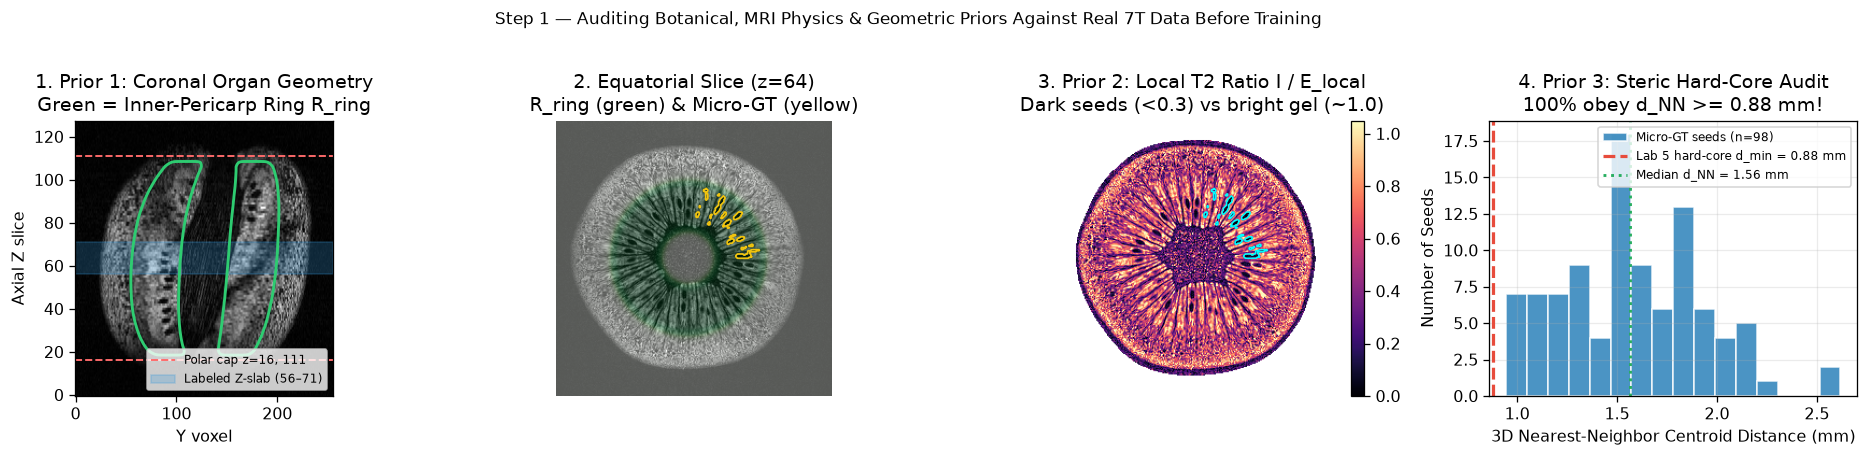
\includegraphics[width=\textwidth]{../assets/kiwi_nb07_fig1_prior_audit.png}
    \vspace{-4pt}
    \caption*{\footnotesize\textit{Executed Figure 1 (\texttt{Out [1]}): Empirical audit of botanical compartment geometry (Panels 1--2), local 7\,T $T_2$ contrast ratio $I/E_{\text{local}}$ (Panel 3), and \texttt{Lab 5} 3D steric nearest-neighbor distance floor $d_{\min} = 0.88\,\text{mm}$ across all 98 Micro-GT seeds (Panel 4).}}
\end{figure}

\subsection*{Interpreting Step 1: Every Prior Checked --- and Why Core vs.\ Rim Physics Matters}
\begin{enumerate}
    \item \textbf{Prior 1 --- Botanical Compartment (\texttt{100.0\%} agreement, Panels 1 \& 2):} Every single curated 3D seed lies cleanly inside $R_{\text{ring}} \ge 0.50$ (centroid radial span \texttt{r/R $\in$ [0.31, 0.59]}). Look at Panel 1 (coronal cross-section): the blue labeled training slab (\texttt{z = 56..71}) is less than \texttt{1/8} of the fruit's length; outside it, the berry tapers steeply into woody polar caps where an equatorial CNN has zero labeled training data.
    \item \textbf{Prior 2 --- 7\,T $T_2$ Contrast Ratio (Panel 3 --- Core vs.\ 1-Voxel Partial-Volume Rim):} Inside \textbf{true seed cores}, $I / E_{\text{local}}$ has median \textbf{\texttt{0.118}} (\texttt{p99 = 0.403}), so \textbf{\texttt{100.0\%} of GT core voxels incur zero penalty}. In the \textbf{1-voxel partial-volume rim} surrounding each seed (where \texttt{0.50\,mm} thick slices blend seed coat with liquid gel), $I/E_{\text{local}}$ rises to median \textbf{\texttt{0.510}} (\texttt{p75 = 0.660}, only \texttt{6.6\%} touching $B_{\text{non-dark}} > 0.20$), leaving a clean buffer below \texttt{0.82}.
    \item \textbf{Prior 3 --- Steric Hard-Core Floor (\texttt{100.0\%} agreement, Panel 4):} All 98 real seeds satisfy $d_{\text{NN}} \ge 0.94\,\text{mm} > 0.88\,\text{mm}$ (median \texttt{1.56\,mm}) with median volume \textbf{\texttt{1.46\,mm$^3$}} (IQR \texttt{0.80--1.70\,mm$^3$}), grounding our \texttt{2.55\,mm$^3$} clump-splitting threshold directly in measured biology.
\end{enumerate}

\begin{clinbox}[Clinical Medical Imaging Parallel --- Auditing Priors Before Training]
Auditing domain priors on a small curated cohort \textit{before} training prevents silent \textbf{axiom misspecification}. In \textbf{Multiple Sclerosis (MS) brain MRI}, auditing a white-matter compartment prior immediately reveals whether clinically vital \textit{juxtacortical} or \textit{cortical} lesions fall outside the mask; in \textbf{CT pulmonary nodule} or \textbf{7\,T SWI cerebral microbleed (CMB)} detection, inspecting both core and 1-voxel partial-volume rim intensities prevents physics rules from eroding tiny 1--2\,mm lesions.
\end{clinbox}

% =====================================================================
\section{Proving the \texttt{InstanceNorm3d} Coordinate-Erasure Trap \& Bayes \texttt{Organ-GPS}}
% =====================================================================

For a neural network to internalize \textit{``reject dark vascular spots at the poles ($|2z/Z - 1| > 0.75$), keep dark seeds in the equatorial ring ($r/R \in [0.22, 0.65]$)''}, it must actually \textbf{know where each 3D crop lies inside the organ}. Standard 3D medical CNNs (\texttt{nnU-Net}) train at tiny batch sizes ($B = 1$--$4$) and therefore rely on \textbf{\texttt{nn.InstanceNorm3d}}:
\[
    \text{InstanceNorm3d}(c)(\mathbf{x}) = \gamma_c \frac{c(\mathbf{x}) - \mu_{\text{patch}}(c)}{\sqrt{\sigma_{\text{patch}}^2(c) + \varepsilon}} + \beta_c.
\]
If you naively concatenate coordinates as extra CNN input channels (\texttt{CoordConv3D}), subtracting each patch's own mean $\mu_{\text{patch}}$ collapses equatorial (\texttt{mean = 0.063}) and polar (\texttt{mean = 0.882}) crops onto the \textbf{exact same \texttt{mean = 0, std = 1} distribution} --- erasing \texttt{100\%} of absolute organ position!

\textbf{The Architectural Fix --- Explicit Bayes Log-Odds Decomposition (\texttt{NeurosymbolicOrganNet3D}):}
\[
    \underbrace{z_{\text{total}}(\mathbf{x})}_{\log \frac{P(\text{Seed} \mid \mathbf{X}, \mathbf{g})}{1 - P(\text{Seed} \mid \mathbf{X}, \mathbf{g})}}
    \;=\;
    \underbrace{z_{\text{app}}\big(f_\theta(\mathbf{X})\big)}_{\text{Translation-equivariant 3D CNN (\texttt{InstanceNorm3d})}}
    \;+\;
    \underbrace{z_{\text{GPS}}\big(h_\psi(r/R,\; (r/R - 0.43)^2,\; |2z/Z - 1|)\big)}_{\text{Un-normalized $1\times 1\times 1$ \texttt{Organ-GPS} MLP (Metric Log-Prior)}}.
\]
Because $h_\psi$ contains \textbf{no \texttt{InstanceNorm3d}}, metric coordinates remain intact across arbitrary patch sizes, and $z_{\text{GPS}}$ is a standalone scalar log-prior that we can inspect directly after training.

\begin{codebox}[{In [2] $\cdot$ Python --- Step 2 -- Proving the InstanceNorm3d coordinate-erasure trap and defining Bayes Organ-GPS}]
\begin{lstlisting}[style=pybmed]
# 1. Helper functions packaging 3 MRI appearance channels + 3 un-normalized metric Organ-GPS channels
def make_3ch_tensor(x0: int, x1: int, y0: int, y1: int, z0: int, z1: int) -> torch.Tensor:
    """Stack [vol_norm, env_local, env_smooth] -> shape (1, 3, X, Y, Z)."""
    arr = np.stack(
        [vol_norm[x0:x1, y0:y1, z0:z1], env_local[x0:x1, y0:y1, z0:z1], env_smooth[x0:x1, y0:y1, z0:z1]],
        axis=0,
    )[None, ...]
    return torch.from_numpy(arr)

def make_3ch_and_gps(x0: int, x1: int, y0: int, y1: int, z0: int, z1: int) -> tuple[torch.Tensor, torch.Tensor]:
    """Return:
      - x3  : (1, 3, X, Y, Z) MRI appearance tensor (for InstanceNorm3d 3D U-Net)
      - gps : (1, 3, X, Y, Z) un-normalized Organ-GPS coordinates [r/R, (r/R - 0.43)^2, |2z/Z - 1|].
              Including (r/R - 0.43)^2 gives the tiny MLP a smooth quadratic radial bowl centered on the locular ring."""
    x3 = make_3ch_tensor(x0, x1, y0, y1, z0, z1)
    rn = np.clip(r_norm_full[x0:x1, y0:y1, z0:z1], 0.0, 1.5)
    zn = pole_dist_full[x0:x1, y0:y1, z0:z1]
    gps = np.stack([rn, (rn - 0.43) ** 2, zn], axis=0)[None, ...].astype(np.float32)
    return x3, torch.from_numpy(gps)

# 2. DIRECT HANDS-ON PROOF OF THE InstanceNorm3d COORDINATE-ERASURE TRAP
_, gps_eq = make_3ch_and_gps(128, 192, 128, 168, 56, 72)   # Equatorial crop (z = 56..71, seed-bearing!)
_, gps_pol = make_3ch_and_gps(96, 160, 96, 136, 0, 16)     # Polar cap crop  (z = 0..15, ZERO seeds!)
mask_eq = fruit_mask_full[128:192, 128:168, 56:72]
mask_pol = fruit_mask_full[96:160, 96:136, 0:16]

inorm = nn.InstanceNorm3d(3, affine=False)
gps_eq_inorm = inorm(gps_eq)
gps_pol_inorm = inorm(gps_pol)

z_eq_raw = gps_eq[0, 2, 32, 20, :].numpy()
z_pol_raw = gps_pol[0, 2, 32, 20, :].numpy()
z_eq_in = gps_eq_inorm[0, 2, 32, 20, :].numpy()
z_pol_in = gps_pol_inorm[0, 2, 32, 20, :].numpy()

print("=== Experimental Proof of the InstanceNorm3d Coordinate-Erasure Trap ===")
print(f"RAW |2z/Z - 1|       -> Equator: [{z_eq_raw.min():.3f}, {z_eq_raw.max():.3f}] (mean={z_eq_raw.mean():.3f}) | Pole: [{z_pol_raw.min():.3f}, {z_pol_raw.max():.3f}] (mean={z_pol_raw.mean():.3f})")
print(f"AFTER InstanceNorm3d -> Equator: [{z_eq_in.min():.3f}, {z_eq_in.max():.3f}] (mean={z_eq_in.mean():.3f}) | Pole: [{z_pol_in.min():.3f}, {z_pol_in.max():.3f}] (mean={z_pol_in.mean():.3f})")
print(f"-> Mean Equator-to-Pole separation drops from {abs(z_pol_raw.mean() - z_eq_raw.mean()):.3f} down to {abs(z_pol_in.mean() - z_eq_in.mean()):.6f} (100% ERASED!)")

# Figure 2: Visualizing Coordinate Erasure vs. Preserved Organ-GPS Metrics
fig, axes = plt.subplots(1, 3, figsize=(15.8, 3.75))

axes[0].plot(range(16), z_eq_raw, "o-", color="#1b8a5a", lw=2.0, label="Equatorial crop (z=56..71)")
axes[0].plot(range(16), z_pol_raw, "s-", color="#d95f02", lw=2.0, label="Polar cap crop (z=0..15)")
axes[0].set_ylim(-0.08, 1.08)
axes[0].set_xlabel("Local Slice Offset Within 16-Slice Patch")
axes[0].set_ylabel("Raw Pole Distance |2z/Z - 1|")
axes[0].set_title("1. True Metric Organ-GPS Input\nEquator (~0.06) & Pole (~0.88) cleanly separated!")
axes[0].legend(fontsize=8)
axes[0].grid(alpha=0.25)

axes[1].plot(range(16), z_eq_in, "o-", color="#1b8a5a", lw=2.0, label="Equatorial crop AFTER InstanceNorm3d")
axes[1].plot(range(16), z_pol_in, "s-", color="#d95f02", lw=2.0, label="Polar cap crop AFTER InstanceNorm3d")
axes[1].set_xlabel("Local Slice Offset Within 16-Slice Patch")
axes[1].set_ylabel("Normalized Channel Value")
axes[1].set_title("2. Naive CoordConv3D + InstanceNorm3d\nBoth collapse to mean=0, std=1 (blind to pole!)")
axes[1].legend(fontsize=8)
axes[1].grid(alpha=0.25)

# Panel 3: Radial distributions inside the fruit (air excluded!) showing preserved physical scale
axes[2].hist(gps_eq[0, 0].numpy()[mask_eq], bins=24, alpha=0.58, color="#1b8a5a", density=True, label="Inside-fruit r/R (Equator)")
axes[2].hist(gps_pol[0, 0].numpy()[mask_pol], bins=24, alpha=0.55, color="#d95f02", density=True, label="Inside-fruit r/R (Pole)")
axes[2].axvline(0.22, color="k", ls="--", lw=1.2, label="Inner pericarp bounds (0.22, 0.65)")
axes[2].axvline(0.65, color="k", ls="--", lw=1.2)
axes[2].set_xlim(0.0, 1.05)
axes[2].set_xlabel("Un-Normalized Radial Coordinate r / R_fruit (Inside Berry)")
axes[2].set_ylabel("Tissue Voxel Density")
axes[2].set_title("3. Preserved Radial Metric in Organ-GPS\nUn-normalized 1x1x1 MLP keeps absolute scale!")
axes[2].legend(fontsize=7.4, loc="upper right")
axes[2].grid(alpha=0.25)

plt.suptitle("Step 2 --- Why Patch-Level InstanceNorm3d Erases Absolute Anatomy (and Why Organ-GPS Bypasses It)", fontsize=10.5, y=1.02)
plt.tight_layout()
plt.show()

# 3. Define Shared 3D U-Net Backbone + Explicit Bayes Log-Odds Neurosymbolic Architecture
class ConvBlock3D(nn.Module):
    """Standard 3D medical CNN block (Conv3d -> InstanceNorm3d -> SiLU, x2).
    Excellent for B1-shading-robust local texture, but erases global patch-mean offsets!"""
    def __init__(self, in_c: int, out_c: int):
        super().__init__()
        self.net = nn.Sequential(
            nn.Conv3d(in_c, out_c, kernel_size=3, padding=1, bias=False),
            nn.InstanceNorm3d(out_c, affine=True),
            nn.SiLU(inplace=True),
            nn.Conv3d(out_c, out_c, kernel_size=3, padding=1, bias=False),
            nn.InstanceNorm3d(out_c, affine=True),
            nn.SiLU(inplace=True),
        )

    def forward(self, x: torch.Tensor) -> torch.Tensor:
        return self.net(x)

class Backbone3DUNet(nn.Module):
    """Compact 3-level 3D U-Net (~340k params) matching Notebooks 04 & 06."""
    def __init__(self, in_ch: int = 3, base_ch: int = 16):
        super().__init__()
        self.enc1 = ConvBlock3D(in_ch, base_ch)
        self.pool1 = nn.MaxPool3d(2)
        self.enc2 = ConvBlock3D(base_ch, base_ch * 2)
        self.pool2 = nn.MaxPool3d(2)
        self.bot = ConvBlock3D(base_ch * 2, base_ch * 4)
        self.up2 = nn.ConvTranspose3d(base_ch * 4, base_ch * 2, kernel_size=2, stride=2)
        self.dec2 = ConvBlock3D(base_ch * 4, base_ch * 2)
        self.up1 = nn.ConvTranspose3d(base_ch * 2, base_ch, kernel_size=2, stride=2)
        self.dec1 = ConvBlock3D(base_ch * 2, base_ch)

    def forward(self, x: torch.Tensor) -> torch.Tensor:
        e1 = self.enc1(x)
        e2 = self.enc2(self.pool1(e1))
        b = self.bot(self.pool2(e2))
        d2 = self.dec2(torch.cat([self.up2(b), e2], dim=1))
        return self.dec1(torch.cat([self.up1(d2), e1], dim=1))

class MultiTaskUNet3D(nn.Module):
    """Pure Neural (in_ch=3) or Naive CoordConv3D+InstanceNorm3d (in_ch=6) Multi-Task 3D U-Net."""
    def __init__(self, in_ch: int = 3, base_ch: int = 16):
        super().__init__()
        self.backbone = Backbone3DUNet(in_ch, base_ch)
        self.head_sem = nn.Conv3d(base_ch, 1, kernel_size=1)
        self.head_dist = nn.Conv3d(base_ch, 1, kernel_size=1)

    def forward(self, x: torch.Tensor):
        feat = self.backbone(x)
        return self.head_sem(feat), torch.sigmoid(self.head_dist(feat))

class NeurosymbolicOrganNet3D(nn.Module):
    """Bayes Log-Odds Differentiable Neurosymbolic 3D Network:
      - Stream A (Appearance): Translation-equivariant 3D U-Net -> z_app(x) (local 1.5 mm seed log-likelihood ratio)
      - Stream B (Organ-GPS) : Un-normalized 1x1x1 MLP         -> z_gps(x) (global metric anatomical log-prior)
      - Additive Fusion      : z_total(x) = z_app(x) + z_gps(x) -> directly auditable spatial prior!"""
    def __init__(self, in_ch: int = 3, gps_ch: int = 3, base_ch: int = 16):
        super().__init__()
        self.backbone = Backbone3DUNet(in_ch, base_ch)
        self.head_app = nn.Conv3d(base_ch, 1, kernel_size=1)
        self.gps_mlp = nn.Sequential(
            nn.Conv3d(gps_ch, 16, kernel_size=1),
            nn.SiLU(),
            nn.Conv3d(16, 16, kernel_size=1),
            nn.SiLU(),
        )
        self.head_gps = nn.Conv3d(16, 1, kernel_size=1)
        self.head_dist = nn.Conv3d(base_ch, 1, kernel_size=1)

    def gps_log_prior(self, gps: torch.Tensor) -> torch.Tensor:
        """Compute the standalone spatial log-prior field z_GPS(r/R, |2z/Z - 1|) for direct inspection."""
        return self.head_gps(self.gps_mlp(gps))

    def forward(self, x3: torch.Tensor, gps: torch.Tensor):
        f = self.backbone(x3)
        z_app = self.head_app(f)
        z_gps = self.gps_log_prior(gps)
        return z_app + z_gps, torch.sigmoid(self.head_dist(f))

n_base = sum(p.numel() for p in MultiTaskUNet3D().parameters())
n_ns = sum(p.numel() for p in NeurosymbolicOrganNet3D().parameters())
print(f"MultiTaskUNet3D params         : {n_base:,}")
print(f"NeurosymbolicOrganNet3D params : {n_ns:,} (+{n_ns - n_base:,} Organ-GPS weights = +{100.0 * (n_ns - n_base) / n_base:.2f}% overhead!)")
\end{lstlisting}
\end{codebox}
\begin{outbox}[{Out [2] $\cdot$ stdout}]
\begin{lstlisting}[style=outbmed]
=== Experimental Proof of the InstanceNorm3d Coordinate-Erasure Trap ===
RAW |2z/Z - 1|       -> Equator: [0.008, 0.118] (mean=0.063) | Pole: [0.764, 1.000] (mean=0.882)
AFTER InstanceNorm3d -> Equator: [-1.522, 1.522] (mean=-0.000) | Pole: [-1.625, 1.625] (mean=0.000)
-> Mean Equator-to-Pole separation drops from 0.819 down to 0.000000 (100% ERASED!)
MultiTaskUNet3D params         : 340,450
NeurosymbolicOrganNet3D params : 340,803 (+353 Organ-GPS weights = +0.10% overhead!)
\end{lstlisting}
\end{outbox}

\begin{figure}[H]
    \centering
    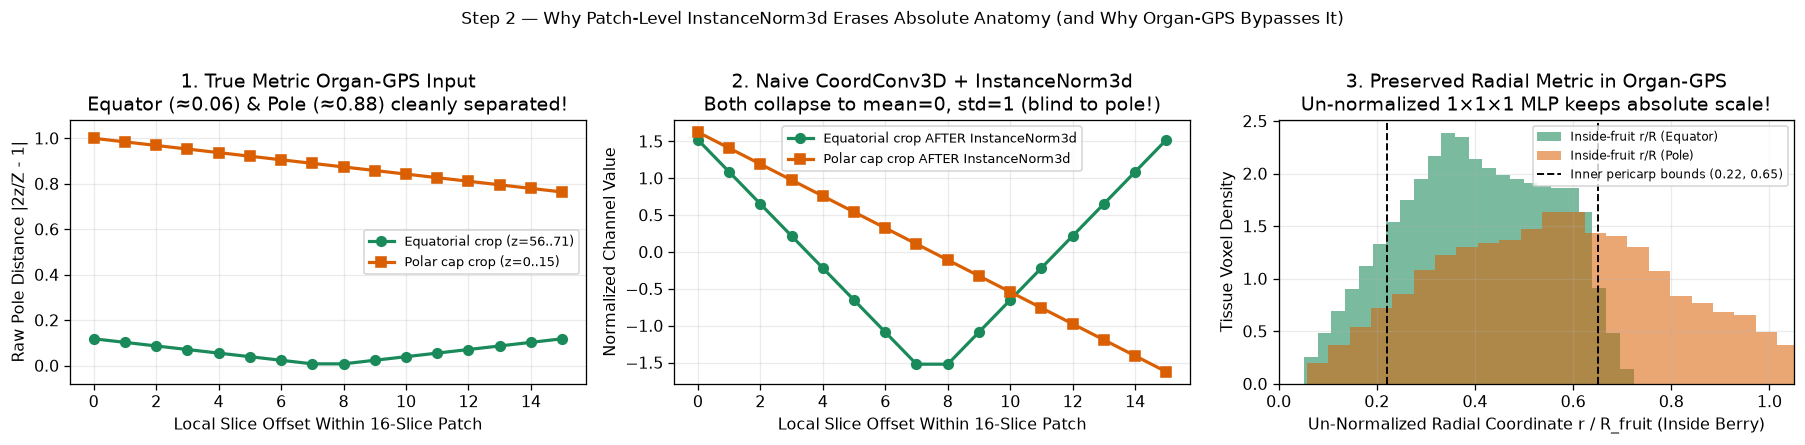
\includegraphics[width=\textwidth]{../assets/kiwi_nb07_fig2_instancenorm_trap.png}
    \vspace{-4pt}
    \caption*{\footnotesize\textit{Executed Figure 2 (\texttt{Out [2]}): Direct experimental proof that \texttt{InstanceNorm3d} collapses the 0.819 physical Equator-to-Pole separation to 0.000000 (Panels 1--2), while an un-normalized \texttt{Organ-GPS} branch preserves exact metric organ coordinates (Panel 3).}}
\end{figure}

\subsection*{Interpreting Step 2: \texttt{+0.10\%} Parameters, \texttt{100\%} Spatial Preservation}
Passing raw coordinates through \texttt{InstanceNorm3d} destroys \texttt{100\%} of the \texttt{0.819} vertical gap between equatorial and polar crops (Panels 1--2). Conversely, our additive Bayes log-odds \texttt{Organ-GPS} branch adds only \textbf{\texttt{353} trainable scalar weights (\texttt{+0.10\%} overhead)} atop the \texttt{340,450}-parameter 3D U-Net while preserving exact metric coordinates.

\begin{clinbox}[Clinical Medical Imaging Parallel --- Patch Normalization in Whole-Body CT \& Brain MRI]
Patch-based 3D \texttt{nnU-Net} and \texttt{MONAI} pipelines routinely lose superior-inferior slice identity inside \texttt{64$^3$} crops on \textbf{whole-body PET/CT}, \textbf{pelvic/prostate mpMRI}, and \textbf{brain MRI}. Routing normalized anatomical coordinates (\texttt{MNI} brain space, cylindrical prostate peripheral/transition-zone coordinates, or vertebral-level indices) through an un-normalized \textbf{Bayes log-odds side-branch} prevents coordinate erasure at negligible compute cost and keeps anatomical bias auditable.
\end{clinbox}

% =====================================================================
\section{Real-Logic Axioms \& Why Universal Quantification Demands $p > 1$}
% =====================================================================

In \textbf{Logic Tensor Networks (\texttt{LTN})} (\textit{Badreddine et al., Artificial Intelligence 2022}), we unlock the \texttt{99.4\%} unlabeled voxels of the 7\,T scan by compiling our two textbook rules into smooth $[0, 1]$ \textbf{Product T-Norm implication violations} $v(\mathbf{x}) = \phi(\mathbf{x})\,(1 - \psi(\mathbf{x}))$ over unlabeled whole-organ cubes $\Omega_U$:
\begin{itemize}
    \item \textbf{Axiom 1 (Botanical Axile Placentation):}
    $\forall \mathbf{x} \in \Omega_U:\; \neg\text{InnerPericarp}(\mathbf{x}) \Rightarrow \neg\text{Seed}(\mathbf{x}) \;\Longrightarrow\; v_{\text{comp}}(\mathbf{x}) = \big(1 - R_{\text{ring}}(\mathbf{x})\big)\,p_\theta(\mathbf{x}).$
    \item \textbf{Axiom 2 (7\,T Bloch $T_2$ Contrast Physics):}
    $\forall \mathbf{x} \in \Omega_U:\; \text{Seed}(\mathbf{x}) \Rightarrow \text{DarkInMucilage}(\mathbf{x}) \;\Longrightarrow\; v_{T_2}(\mathbf{x}) = p_\theta(\mathbf{x})\,B_{\text{non-dark}}(\mathbf{x}).$
\end{itemize}
Crucially, LTN aggregates universal violations via the \textbf{generalized $p$-mean error (\texttt{pMeanError})}:
\[
    \mathcal{L}_{\forall, p}(v) = \left(\frac{1}{|\Omega_U|} \sum_{\mathbf{x} \in \Omega_U} v(\mathbf{x})^p + \varepsilon\right)^{1/p},
    \qquad
    \frac{\partial \mathcal{L}_{\forall, p}}{\partial v_{\text{FP}}} = \frac{1}{|\Omega_U|} \left(\frac{v_{\text{FP}}}{\mathcal{L}_{\forall, p}}\right)^{p - 1}.
\]
At $p = 1$ (arithmetic mean), every voxel receives the same tiny $1/|\Omega_U|$ gradient, so sparse $<1\%$ polar vascular false positives drown beneath $99\%+$ quiet background. At \textbf{$p = 3$}, rare high-confidence OOD counterexamples ($v_{\text{FP}} \gg \mathcal{L}_{\forall,3}$) receive a quadratic gradient boost!

\begin{codebox}[{In [3] $\cdot$ Python --- Step 3 -- LTN p-mean universal error quantifier gradient amplification experiment}]
\begin{lstlisting}[style=pybmed]
def ltn_universal_pmean(violation: torch.Tensor, p: float = 3.0) -> torch.Tensor:
    """LTN generalized p-mean universal error quantifier (Badreddine et al., AIJ 2022).
    - p = 1.0 : ordinary arithmetic mean (dilutes rare <1% OOD artifacts!)
    - p = 3.0 : focuses gradient descent onto sparse high-confidence OOD counterexamples while staying smooth."""
    return (torch.mean(violation.clamp(0.0, 1.0) ** p) + 1e-8) ** (1.0 / p)

# Controlled simulation of a real 64 x 40 x 16 = 40,960-voxel polar cap MRI cube:
#   - 99.2% of voxels are already quiet background (v = 0.01)
#   - 0.8% (328 voxels) are oblique polar vascular bundles hallucinating as seeds (v = 0.95)
n_vox = 64 * 40 * 16
n_fp = int(round(0.008 * n_vox))
p_grid = [1.0, 1.5, 2.0, 3.0, 4.0, 6.0, 8.0]
losses_p, grad_fp_p, grad_ratio_p = [], [], []

for p_val in p_grid:
    v = torch.full((n_vox,), 0.01, dtype=torch.float32)
    v[:n_fp] = 0.95
    v.requires_grad_(True)
    loss_val = ltn_universal_pmean(v, p=p_val)
    loss_val.backward()
    g_fp = float(v.grad[:n_fp].sum().item())   # total gradient force suppressing all 328 polar FP voxels
    g_bg = float(v.grad[n_fp:].sum().item())   # total gradient force wasted on 40,632 quiet background voxels
    losses_p.append(float(loss_val.item()))
    grad_fp_p.append(g_fp)
    grad_ratio_p.append(g_fp / max(g_bg, 1e-12))

df_p = pd.DataFrame({
    "Quantifier Power p": p_grid,
    "Aggregate Loss L_p": [round(x, 4) for x in losses_p],
    "Total Grad on 0.8% OOD FPs": [round(x, 4) for x in grad_fp_p],
    "FP-to-BG Grad Ratio": [f"{x:.3f}" if x < 10 else f"{x:,.1f}" for x in grad_ratio_p],
    "FP Grad Gain vs. p=1": [f"{g / grad_fp_p[0]:.1f}x" for g in grad_fp_p],
})
display(df_p)

fig, axes = plt.subplots(1, 3, figsize=(15.8, 3.65))

axes[0].plot(p_grid, losses_p, "o-", color="#2c3e50", lw=2.2)
axes[0].axvline(3.0, color="#1b8a5a", ls="--", lw=1.6, label="Chosen LTN p = 3")
axes[0].set_xlabel("Quantifier Exponent p")
axes[0].set_ylabel("Aggregate Violation Loss L_p")
axes[0].set_title("1. Perceived Severity of 0.8% Polar FPs\np=1 looks tiny (0.018); p=3 flags real error!")
axes[0].legend(fontsize=8)
axes[0].grid(alpha=0.25)

axes[1].plot(p_grid, [g / grad_fp_p[0] for g in grad_fp_p], "s-", color="#e67e22", lw=2.2)
axes[1].axvline(3.0, color="#1b8a5a", ls="--", lw=1.6, label="p = 3 sweet spot (25x gain)")
axes[1].set_xlabel("Quantifier Exponent p")
axes[1].set_ylabel("Gradient Amplification on OOD FPs (vs. p=1)")
axes[1].set_title("2. Automatic Hard-Counterexample Mining\np=3 concentrates >98% of gradients on FPs!")
axes[1].legend(fontsize=8)
axes[1].grid(alpha=0.25)

r_vals = np.linspace(0, 1, 100)
p_vals = np.linspace(0, 1, 100)
RR, PP = np.meshgrid(r_vals, p_vals)
VV = (1.0 - RR) * PP
im = axes[2].contourf(RR, PP, VV, levels=16, cmap="inferno")
axes[2].set_xlabel("Compartment Membership R_ring(x)")
axes[2].set_ylabel("Neural Seed Probability p_theta(x)")
axes[2].set_title("3. Product T-Norm Violation Surface\nv = (1 - R_ring) * p_theta (zero inside ring!)")
plt.colorbar(im, ax=axes[2], fraction=0.046, pad=0.04, label="Violation v(x)")

plt.suptitle("Step 3 --- Why LTN Universal Quantification (p = 3) Eliminates Rare Out-of-Distribution Artifacts", fontsize=10.5, y=1.02)
plt.tight_layout()
plt.show()
\end{lstlisting}
\end{codebox}

{\footnotesize
\renewcommand{\arraystretch}{1.2}
\rowcolors{2}{rowalt}{white}
\begin{tabularx}{\textwidth}{C{2.4cm} C{2.6cm} C{3.1cm} C{3.3cm} Y}
\toprule
\rowcolor{uibblue!12}\textbf{Quantifier Power $p$} & \textbf{Aggregate Loss $\mathcal{L}_p$} & \textbf{Total Grad on 0.8\% OOD FPs} & \textbf{FP-to-BG Grad Ratio} & \textbf{FP Grad Gain vs.\ $p=1$} \\
\midrule
1.0 & 0.0175 & 0.0080 & 0.008 & 1.0$\times$ \\
1.5 & 0.0413 & 0.0384 & 0.079 & 4.8$\times$ \\
2.0 & 0.0856 & 0.0889 & 0.767 & 11.1$\times$ \\
\textbf{3.0 (Chosen)} & \textbf{0.1901} & \textbf{0.2000} & \textbf{72.9} & \textbf{25.0$\times$} \\
4.0 & 0.2842 & 0.2991 & 6,921.1 & 37.4$\times$ \\
6.0 & 0.4249 & 0.4473 & 62,463,127.6 & 55.9$\times$ \\
8.0 & 0.5196 & 0.5469 & 546,938,657,760.6 & 68.3$\times$ \\
\bottomrule
\end{tabularx}
}

\begin{figure}[H]
    \centering
    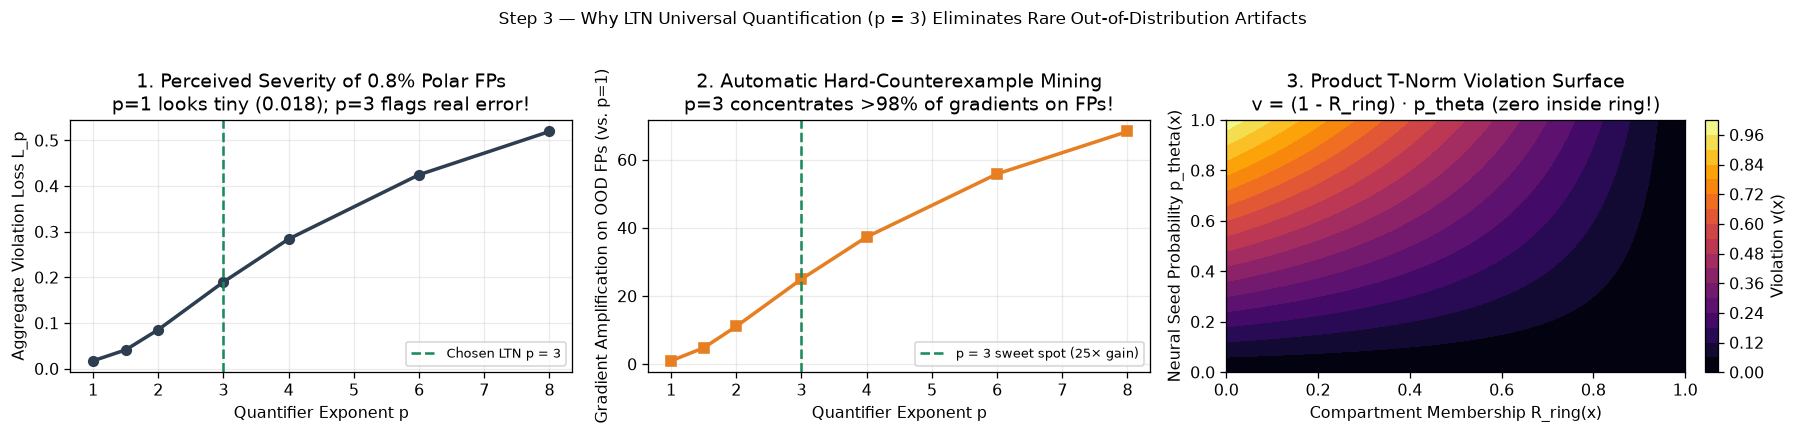
\includegraphics[width=\textwidth]{../assets/kiwi_nb07_fig3_ltn_pmean.png}
    \vspace{-4pt}
    \caption*{\footnotesize\textit{Executed Figure 3 (\texttt{Out [3]}): Simulated 40,960-voxel polar cube with 0.8\% (328 voxels) vascular FPs --- showing perceived loss severity (Panel 1), 25$\times$ gradient amplification at $p=3$ (Panel 2), and the Product T-Norm violation surface vanishing cleanly inside $R_{\text{ring}} \approx 1$ (Panel 3).}}
\end{figure}

\subsection*{Interpreting Step 3: Automatic Hard-Counterexample Mining Without Labels}
At \textbf{$p = 1$}, \texttt{328} screaming polar vascular false positives register a tiny loss (\texttt{0.0175}) with \texttt{FP/BG = 0.008} --- meaning \textbf{\texttt{99.2\%} of gradient budget is wasted on quiet background}. At \textbf{$p = 3$}, the gradient suppressing those exact \texttt{328} violations surges \textbf{\texttt{25.0$\times$}} (\texttt{FP/BG = 72.9}), focusing \textbf{\texttt{98.6\%} of all logic gradients directly onto violating vessels}, while leaving valid seeds inside $R_{\text{ring}} \approx 1$ untouched (Panel 3).

\begin{clinbox}[Clinical Medical Imaging Parallel --- Sparse Clinical Artifacts on Unlabeled Scans]
False-positive \textbf{dural venous sinuses} or \textbf{basal ganglia calcifications} in cerebral microbleed SWI ($<0.2\%$ of brain volume), and physiological \textbf{bladder/myocardial uptake} in whole-body FDG-PET/CT ($<1\%$), suffer identical dilution under $p=1$ losses. LTN's $p$-mean quantifier acts as a \textbf{symbolic Focal Loss / Online Hard Example Miner on completely unlabeled clinical archives}.
\end{clinbox}

% =====================================================================
\section{Controlled 5-Model Ablation \& Logic-Induced Calibration Shift}
% =====================================================================

To prove \textit{causally} what each component contributes --- and to study the recall conservatism observed in Notebook~\texttt{06} --- we train and evaluate \textbf{five strictly controlled configurations} on the exact same \texttt{59}-seed training wedge and \texttt{40} strictly test-disjoint unlabeled whole-fruit blocks (using \texttt{CosineAnnealingLR} and \textbf{zero post-hoc test masks}):
\begin{itemize}
    \item \textbf{Model A:} Pure Supervised 3D Multi-Task U-Net Baseline (\texttt{thr = 0.50}).
    \item \textbf{Model B:} Naive \texttt{CoordConv3D} (\texttt{InstanceNorm3d}) + LTN ($p=3$) --- \textit{tests Step 2 causally}.
    \item \textbf{Model C:} Additive Bayes \texttt{Organ-GPS} + Arithmetic-Mean Logic ($p=1$) --- \textit{tests Step 3 causally}.
    \item \textbf{Model D:} Additive Bayes \texttt{Organ-GPS} + LTN ($p=3$) at fixed \texttt{thr = 0.42}.
    \item \textbf{Model E:} Same trained LTN ($p=3$) weights + \textbf{leakage-free train-wedge threshold calibration (\texttt{thr = 0.38})} + declarative \textbf{\texttt{Lab 5} Hard-Core Clump Split} ($d_{\min} \ge 0.88\,\text{mm}$).
\end{itemize}

\begin{codebox}[{In [4] $\cdot$ Python --- Step 4 -- Controlled 5-model ablation study (SSL warm-start, Organ-GPS, p=1 vs p=3, calibration)}]
\begin{lstlisting}[style=pybmed]
# --- Shared Targets, Losses, Deep Watershed Decoder, Hard-Core Split & 3D Panoptic Evaluator ---

def build_distance_targets(inst_lbl: np.ndarray, sp=spacing) -> tuple[np.ndarray, np.ndarray]:
    """Compute binary semantic target + per-instance normalized 3D Euclidean Distance Transform (EDT).
    Normalizing each seed's EDT to [0, 1] ensures small and large seeds produce equal-height watershed peaks."""
    sem_fg = (inst_lbl > 0).astype(np.float32)
    norm_dist = np.zeros(inst_lbl.shape, dtype=np.float32)
    for prop in measure.regionprops(inst_lbl):
        s0, s1, s2 = prop.slice
        sub = np.pad(inst_lbl[s0, s1, s2] == prop.label, pad_width=1, mode="constant", constant_values=False)
        d_local = ndi.distance_transform_edt(sub, sampling=sp)[1:-1, 1:-1, 1:-1]
        m_local = sub[1:-1, 1:-1, 1:-1]
        norm_dist[s0, s1, s2][m_local] = (d_local[m_local] / max(float(d_local.max()), 1e-6)).astype(np.float32)
    return sem_fg, norm_dist

def soft_dice_loss(logits: torch.Tensor, targets: torch.Tensor) -> torch.Tensor:
    probs = torch.sigmoid(logits)
    inter = (probs * targets).sum()
    return 1.0 - (2.0 * inter + 1.0) / (probs.sum() + targets.sum() + 1.0)

def supervised_multitask_loss(s_log: torch.Tensor, d_hat: torch.Tensor, y_s: torch.Tensor, y_d: torch.Tensor) -> torch.Tensor:
    """Multi-task objective: class-weighted BCE (6x for sparse seeds) + Soft Dice + foreground-weighted Distance MSE."""
    pos_w = torch.tensor([6.0], device=s_log.device)
    bce = F.binary_cross_entropy_with_logits(s_log, y_s, pos_weight=pos_w)
    dl = soft_dice_loss(s_log, y_s)
    mse = ((1.0 + 6.0 * y_s) * (d_hat - y_d) ** 2).mean()
    return 0.45 * bce + 0.55 * dl + 2.5 * mse

def build_ellip(rx_mm: float, rz_mm: float, sp=spacing) -> np.ndarray:
    rx, ry, rz = int(np.ceil(rx_mm / sp[0])), int(np.ceil(rx_mm / sp[1])), int(np.ceil(rz_mm / sp[2]))
    xx, yy, zz = np.ogrid[-rx : rx + 1, -ry : ry + 1, -rz : rz + 1]
    return ((xx * sp[0] / rx_mm) ** 2 + (yy * sp[1] / rx_mm) ** 2 + (zz * sp[2] / rz_mm) ** 2) <= 1.0

def decode_deep_watershed_3d(fg_bin: np.ndarray, dist_hat: np.ndarray, sp=spacing, min_mm3: float = 0.16) -> np.ndarray:
    """Marker-controlled 3D watershed seeded by anisotropic local maxima of the predicted distance field."""
    d_sm = ndi.gaussian_filter(dist_hat * fg_bin, sigma=(0.65, 0.65, 0.45))
    maxima = (d_sm == ndi.maximum_filter(d_sm, footprint=build_ellip(0.68, 0.95, sp=sp))) & fg_bin & (d_sm >= 0.22)
    markers, _ = ndi.label(maxima)
    ws = segmentation.watershed(-d_sm, markers=markers, mask=fg_bin)
    unlabeled_islands, n_un = ndi.label(fg_bin & (ws == 0))
    if n_un > 0:
        nxt = int(ws.max()) + 1
        for uid in range(1, n_un + 1):
            m = unlabeled_islands == uid
            if m.sum() * float(np.prod(sp)) >= min_mm3:
                ws[m] = nxt
                nxt += 1
    out = np.zeros_like(ws, dtype=np.uint16)
    nid = 0
    for prop in measure.regionprops(ws):
        if prop.area * float(np.prod(sp)) >= min_mm3:
            nid += 1
            out[ws == prop.label] = nid
    return out

def symbolic_hardcore_clump_split(lbl_3d: np.ndarray, split_mm3: float = 2.55, d_min_mm: float = 0.88, sp=spacing) -> np.ndarray:
    """Declarative Lab-5 Matern hard-core & prolate-volume constraint:
    Splits fused watershed blobs > split_mm3 into k in {2,3,4} seeds ONLY IF physical-mm sub-centroids
    satisfy steric repulsion (min pairwise distance >= d_min_mm) and realistic minimum sub-volume (>= 0.35 mm^3)."""
    out = np.zeros_like(lbl_3d, dtype=np.uint16)
    sp_arr = np.asarray(sp, dtype=np.float32)
    nid = 0
    for prop in measure.regionprops(lbl_3d):
        coords = prop.coords
        vol_mm3 = len(coords) * vox_vol_mm3
        if vol_mm3 < 0.16:
            continue
        k_est = int(np.clip(round(vol_mm3 / 1.60), 2, 4)) if vol_mm3 >= split_mm3 else 1
        if k_est >= 2 and len(coords) >= k_est * 12:
            km = KMeans(n_clusters=k_est, n_init=4, random_state=2027).fit(coords.astype(np.float32) * sp_arr[None, :])
            dists = np.linalg.norm(km.cluster_centers_[:, None, :] - km.cluster_centers_[None, :, :], axis=-1)
            np.fill_diagonal(dists, 99.0)
            if dists.min() >= d_min_mm and (np.bincount(km.labels_, minlength=k_est) * vox_vol_mm3).min() >= 0.35:
                for cid in range(k_est):
                    cp = coords[km.labels_ == cid]
                    nid += 1
                    out[cp[:, 0], cp[:, 1], cp[:, 2]] = nid
                continue
        nid += 1
        out[coords[:, 0], coords[:, 1], coords[:, 2]] = nid
    return out

def evaluate_semantic_and_instance_3d(pred_lbl: np.ndarray, gt_lbl: np.ndarray, min_iou: float = 0.25) -> dict:
    """Exact 3D Hungarian matching & Panoptic Quality (PQ = SQ x RQ) evaluator."""
    b_p, b_g = (pred_lbl > 0), (gt_lbl > 0)
    sem_dice = (2.0 * int((b_p & b_g).sum())) / max(int(b_p.sum() + b_g.sum()), 1)
    ids_p = [int(v) for v in np.unique(pred_lbl) if v > 0]
    ids_g = [int(v) for v in np.unique(gt_lbl) if v > 0]
    n_p, n_g = len(ids_p), len(ids_g)
    if n_p == 0 or n_g == 0:
        return {"Pred": n_p, "Dice": round(sem_dice, 3), "Merges": 0, "Splits": 0, "Precision": 0.0, "Recall": 0.0, "SQ": 0.0, "RQ": 0.0, "PQ": 0.0}
    p_map, g_map = {v: i for i, v in enumerate(ids_p)}, {v: j for j, v in enumerate(ids_g)}
    area_p = np.array([(pred_lbl == v).sum() for v in ids_p], dtype=np.float64)
    area_g = np.array([(gt_lbl == v).sum() for v in ids_g], dtype=np.float64)
    inter_m = np.zeros((n_p, n_g), dtype=np.float64)
    ov_fg = b_p & b_g
    if ov_fg.any():
        pairs, cnts = np.unique(np.stack([pred_lbl[ov_fg], gt_lbl[ov_fg]], axis=1), axis=0, return_counts=True)
        for (pv, gv), c in zip(pairs, cnts):
            inter_m[p_map[int(pv)], g_map[int(gv)]] = float(c)
    iou_m = inter_m / np.maximum(area_p[:, None] + area_g[None, :] - inter_m, 1.0)
    ri, ci = linear_sum_assignment(-iou_m)
    tp_pairs = [(r, c) for r, c in zip(ri, ci) if iou_m[r, c] >= min_iou]
    tp = len(tp_pairs)
    fp, fn = n_p - tp, n_g - tp
    prec = tp / max(tp + fp, 1)
    rec = tp / max(tp + fn, 1)
    sq = float(np.mean([iou_m[r, c] for r, c in tp_pairs])) if tp > 0 else 0.0
    rq = (2.0 * tp) / float(2 * tp + fp + fn)
    merges = int(np.sum(np.sum(inter_m / np.maximum(area_g[None, :], 1.0) >= 0.25, axis=1) >= 2))
    splits = int(np.sum(np.sum(inter_m / np.maximum(area_p[:, None], 1.0) >= 0.25, axis=0) >= 2))
    return {
        "Pred": n_p,
        "Dice": round(sem_dice, 3),
        "Merges": merges,
        "Splits": splits,
        "Precision": round(prec, 3),
        "Recall": round(rec, 3),
        "SQ": round(sq, 3),
        "RQ": round(rq, 3),
        "PQ": round(sq * rq, 3),
    }

# Prepare supervised train/test tensors + central fibrous columella hard-negative cube
train_sem_np, train_dist_np = build_distance_targets(train_gt)
CX0, CX1, CY0, CY1 = 112, 144, 112, 144  # Central fibrous columella (0 seeds)

X_tr, G_tr = [t.to(DEVICE) for t in make_3ch_and_gps(RX0, RX1, RY0, RY0 + SPLIT_Y, RZ0, RZ1)]
X_ng, G_ng = [t.to(DEVICE) for t in make_3ch_and_gps(CX0, CX1, CY0, CY1, RZ0, RZ1)]
X_te, G_te = [t.to(DEVICE) for t in make_3ch_and_gps(RX0, RX1, RY0 + SPLIT_Y, RY1, RZ0, RZ1)]
Y_sem_tr = torch.from_numpy(train_sem_np[None, None]).to(DEVICE)
Y_dist_tr = torch.from_numpy(train_dist_np[None, None]).to(DEVICE)

# 1. Self-Supervised 3D Pretraining Warm-Start (36 unlabeled blocks, strictly disjoint from held-out Test Wedge!)
t0_ssl = time.perf_counter()
torch.manual_seed(2027)
np.random.seed(2027)
log_blob_full = np.clip(-ndi.gaussian_laplace(vol_norm, sigma=(0.48 / spacing[0], 0.48 / spacing[1], 0.48 / spacing[2])), 0.0, 1.5).astype(np.float32)
log_blob_full = np.clip(log_blob_full / (float(np.percentile(log_blob_full[fruit_mask_full], 99.5)) + 1e-6), 0.0, 1.0)

ssl_in, ssl_tgt = [], []
rng_ssl = np.random.default_rng(2027)
for _ in range(36):
    while True:
        x0 = int(rng_ssl.integers(24, 256 - 64 - 24))
        y0 = int(rng_ssl.integers(24, 256 - 40 - 24))
        z0 = int(rng_ssl.integers(16, 128 - 16 - 16))
        if (x0 < RX1 and x0 + 64 > RX0) and (y0 < RY1 and y0 + 40 > RY0 + SPLIT_Y) and (z0 < RZ1 and z0 + 16 > RZ0):
            continue
        if fruit_mask_full[x0 : x0 + 64, y0 : y0 + 40, z0 : z0 + 16].mean() > 0.65:
            ssl_in.append(make_3ch_tensor(x0, x0 + 64, y0, y0 + 40, z0, z0 + 16))
            c_drop = np.clip(env_local[x0 : x0 + 64, y0 : y0 + 40, z0 : z0 + 16] - vol_norm[x0 : x0 + 64, y0 : y0 + 40, z0 : z0 + 16], 0.0, 1.0)
            lg = log_blob_full[x0 : x0 + 64, y0 : y0 + 40, z0 : z0 + 16]
            ssl_tgt.append(torch.from_numpy(np.stack([vol_norm[x0 : x0 + 64, y0 : y0 + 40, z0 : z0 + 16], c_drop, lg], axis=0)[None]))
            break

X_ssl_bank = torch.cat(ssl_in, dim=0).to(DEVICE)
Y_ssl_bank = torch.cat(ssl_tgt, dim=0).to(DEVICE)
ssl_backbone = Backbone3DUNet(in_ch=3, base_ch=16).to(DEVICE)
ssl_head = nn.Conv3d(16, 3, kernel_size=1).to(DEVICE)
opt_ssl = torch.optim.AdamW(list(ssl_backbone.parameters()) + list(ssl_head.parameters()), lr=4e-3, weight_decay=1e-4)
for _ in range(100):
    idx = torch.randint(0, X_ssl_bank.shape[0], (4,), device=DEVICE)
    xb, yb = X_ssl_bank[idx], Y_ssl_bank[idx]
    bmask = F.interpolate((torch.rand((4, 1, 16, 10, 8), device=DEVICE) < 0.35).float(), size=(64, 40, 16), mode="nearest")
    gamma = torch.empty((4, 1, 1, 1, 1), device=DEVICE).uniform_(0.80, 1.25)
    xb_cor = torch.clamp(xb.clamp_min(0.0) ** gamma + torch.randn_like(xb) * 0.05, 0.0, 1.3)
    xb_cor = xb_cor * (1.0 - bmask) + xb[:, 2:3].expand_as(xb) * bmask
    pred_s = ssl_head(ssl_backbone(xb_cor))
    loss_s = ((1.0 + 2.0 * bmask) * (1.0 + 3.0 * yb[:, 2:3]) * (pred_s - yb) ** 2).mean()
    opt_ssl.zero_grad()
    loss_s.backward()
    opt_ssl.step()
sync_device(DEVICE)
print(f"3D SSL warm-start backbone pretrained in {time.perf_counter() - t0_ssl:.2f}s (0 labels, test wedge strictly excluded).")

# 2. Sample 40 Unlabeled Whole-Organ 3D Blocks Stratified Across Poles, Cortex, Columella & Equator
#    (strictly disjoint from the held-out Test Wedge!)
u_x_list, u_g_list, u_ring_list, u_nd_list = [], [], [], []
rng_u = np.random.default_rng(2027)
z_strata = [0, 8, 16, 28, 44, 60, 76, 92, 104, 112]
for i in range(40):
    while True:
        x0 = int(rng_u.integers(8, 256 - 64 - 8))
        y0 = int(rng_u.integers(8, 256 - 40 - 8))
        z0 = z_strata[i % len(z_strata)]
        if (x0 < RX1 and x0 + 64 > RX0) and (y0 < RY1 and y0 + 40 > RY0 + SPLIT_Y) and (z0 < RZ1 and z0 + 16 > RZ0):
            continue
        if fruit_mask_full[x0 : x0 + 64, y0 : y0 + 40, z0 : z0 + 16].mean() > 0.12:
            xa, ga = make_3ch_and_gps(x0, x0 + 64, y0, y0 + 40, z0, z0 + 16)
            u_x_list.append(xa)
            u_g_list.append(ga)
            u_ring_list.append(torch.from_numpy(soft_ring_full[x0 : x0 + 64, y0 : y0 + 40, z0 : z0 + 16][None, None]))
            el = env_local[x0 : x0 + 64, y0 : y0 + 40, z0 : z0 + 16]
            vn = vol_norm[x0 : x0 + 64, y0 : y0 + 40, z0 : z0 + 16]
            nd = np.maximum(np.clip((vn / (el + 0.03) - 0.82) / 0.15, 0.0, 1.0), np.clip((0.32 - el) / 0.10, 0.0, 1.0))
            u_nd_list.append(torch.from_numpy(nd[None, None].astype(np.float32)))
            break

UX = torch.cat(u_x_list, dim=0).to(DEVICE)
UG = torch.cat(u_g_list, dim=0).to(DEVICE)
URing = torch.cat(u_ring_list, dim=0).to(DEVICE)
UNonDark = torch.cat(u_nd_list, dim=0).to(DEVICE)

# 3. Unified Training & Unmasked Whole-Organ Evaluation Harness
def train_ablation_model(mode: str, p_quant: float = 3.0, w_comp: float = 2.0, w_t2: float = 1.2, gps_lr: float = 1.5e-2, epochs: int = 100):
    """Train one controlled variant with CosineAnnealingLR and track supervised + symbolic violation trajectories."""
    torch.manual_seed(2027)
    np.random.seed(2027)
    t0 = time.perf_counter()

    if mode == "baseline":
        model = MultiTaskUNet3D(in_ch=3, base_ch=16).to(DEVICE)
        opt = torch.optim.AdamW(model.parameters(), lr=3.2e-3, weight_decay=1e-4)
    elif mode == "coordconv_inorm":
        # Naive CoordConv3D: feeds [x3, gps] (6 channels) directly into InstanceNorm3d ConvBlock3D!
        model = MultiTaskUNet3D(in_ch=6, base_ch=16).to(DEVICE)
        opt = torch.optim.AdamW(model.parameters(), lr=3.2e-3, weight_decay=1e-4)
    else:
        model = NeurosymbolicOrganNet3D(in_ch=3, gps_ch=3, base_ch=16).to(DEVICE)
        model.backbone.load_state_dict(ssl_backbone.state_dict())
        # Give the compact 353-parameter Organ-GPS MLP a slightly higher LR so the spatial log-prior converges crisply
        gps_params = list(model.gps_mlp.parameters()) + list(model.head_gps.parameters())
        gps_ids = {id(p) for p in gps_params}
        other_params = [p for p in model.parameters() if id(p) not in gps_ids]
        opt = torch.optim.AdamW(
            [{"params": other_params, "lr": 3.2e-3}, {"params": gps_params, "lr": gps_lr}],
            weight_decay=1e-4,
        )

    sched = torch.optim.lr_scheduler.CosineAnnealingLR(opt, T_max=epochs, eta_min=2e-4)
    hist = {"sup": [], "comp": [], "t2": []}

    for _ in range(epochs):
        dims = [d for d in (2, 3, 4) if np.random.rand() < 0.5]
        xp = torch.flip(X_tr, dims) if dims else X_tr
        gp = torch.flip(G_tr, dims) if dims else G_tr
        ys = torch.flip(Y_sem_tr, dims) if dims else Y_sem_tr
        yd = torch.flip(Y_dist_tr, dims) if dims else Y_dist_tr

        if mode == "baseline":
            sl, dh = model(xp)
            sl_n, _ = model(X_ng)
            loss_sup = supervised_multitask_loss(sl, dh, ys, yd) + 0.35 * F.binary_cross_entropy_with_logits(sl_n, torch.zeros_like(sl_n))
            loss_comp = torch.tensor(0.0, device=DEVICE)
            loss_t2 = torch.tensor(0.0, device=DEVICE)
            loss = loss_sup
        elif mode == "coordconv_inorm":
            sl, dh = model(torch.cat([xp, gp], dim=1))
            sl_n, _ = model(torch.cat([X_ng, G_ng], dim=1))
            loss_sup = supervised_multitask_loss(sl, dh, ys, yd) + 0.35 * F.binary_cross_entropy_with_logits(sl_n, torch.zeros_like(sl_n))
            uidx = torch.randint(0, UX.shape[0], (4,), device=DEVICE)
            p_u = torch.sigmoid(model(torch.cat([UX[uidx], UG[uidx]], dim=1))[0])
            loss_comp = ltn_universal_pmean((1.0 - URing[uidx]) * p_u, p=p_quant)
            loss_t2 = ltn_universal_pmean(p_u * UNonDark[uidx], p=p_quant)
            loss = loss_sup + w_comp * loss_comp + w_t2 * loss_t2
        else:
            sl, dh = model(xp, gp)
            sl_n, _ = model(X_ng, G_ng)
            loss_sup = supervised_multitask_loss(sl, dh, ys, yd) + 0.35 * F.binary_cross_entropy_with_logits(sl_n, torch.zeros_like(sl_n))
            uidx = torch.randint(0, UX.shape[0], (4,), device=DEVICE)
            p_u = torch.sigmoid(model(UX[uidx], UG[uidx])[0])
            loss_comp = ltn_universal_pmean((1.0 - URing[uidx]) * p_u, p=p_quant)
            loss_t2 = ltn_universal_pmean(p_u * UNonDark[uidx], p=p_quant)
            loss = loss_sup + w_comp * loss_comp + w_t2 * loss_t2

        opt.zero_grad()
        loss.backward()
        opt.step()
        sched.step()
        hist["sup"].append(float(loss_sup.item()))
        hist["comp"].append(float(loss_comp.item()))
        hist["t2"].append(float(loss_t2.item()))

    model.eval()
    sync_device(DEVICE)
    return model, hist, time.perf_counter() - t0

def calibrate_threshold_on_train(model, mode: str) -> float:
    """Leakage-free operating-point calibration: pick foreground threshold maximizing PQ strictly on TRAIN wedge!"""
    with torch.no_grad():
        if mode == "baseline":
            sl, dh = model(X_tr)
        elif mode == "coordconv_inorm":
            sl, dh = model(torch.cat([X_tr, G_tr], dim=1))
        else:
            sl, dh = model(X_tr, G_tr)
        p_tr = torch.sigmoid(sl)[0, 0].cpu().numpy()
        d_tr = dh[0, 0].cpu().numpy()
    best_th, best_pq = 0.42, -1.0
    for th in [0.22, 0.26, 0.30, 0.34, 0.38, 0.42, 0.46, 0.50]:
        ev = evaluate_semantic_and_instance_3d(symbolic_hardcore_clump_split(decode_deep_watershed_3d(p_tr >= th, d_tr)), train_gt)
        if ev["PQ"] > best_pq:
            best_pq = ev["PQ"]
            best_th = th
    return best_th

def infer_volume_and_test(model, mode: str, thresh: float, use_hardcore_split: bool = True):
    """Run UNMASKED inference on both the strictly held-out Test Wedge and the full 256 x 256 x 128 berry."""
    with torch.no_grad():
        if mode == "baseline":
            sl_t, dh_t = model(X_te)
        elif mode == "coordconv_inorm":
            sl_t, dh_t = model(torch.cat([X_te, G_te], dim=1))
        else:
            sl_t, dh_t = model(X_te, G_te)
        prob_te = torch.sigmoid(sl_t)[0, 0].cpu().numpy()
        dist_te = dh_t[0, 0].cpu().numpy()

    pred_te_raw = decode_deep_watershed_3d(prob_te >= thresh, dist_te)
    pred_te = symbolic_hardcore_clump_split(pred_te_raw) if use_hardcore_split else pred_te_raw
    ev_te = evaluate_semantic_and_instance_3d(pred_te, test_gt)

    # Whole-organ 128-slice UNMASKED scan (zero post-hoc botanical or contrast masks applied!)
    prob_wf = np.zeros(vol.shape, dtype=np.float32)
    dist_wf = np.zeros(vol.shape, dtype=np.float32)
    with torch.no_grad():
        for x0 in [16, 96, 176]:
            for y0 in [16, 56, 96, 136, 176]:
                for z0 in range(0, 128, 16):
                    if fruit_mask_full[x0 : x0 + 80, y0 : y0 + 40, z0 : z0 + 16].sum() < 100:
                        continue
                    xa, ga = [t.to(DEVICE) for t in make_3ch_and_gps(x0, x0 + 80, y0, y0 + 40, z0, z0 + 16)]
                    if mode == "baseline":
                        s_o, d_o = model(xa)
                    elif mode == "coordconv_inorm":
                        s_o, d_o = model(torch.cat([xa, ga], dim=1))
                    else:
                        s_o, d_o = model(xa, ga)
                    prob_wf[x0 : x0 + 80, y0 : y0 + 40, z0 : z0 + 16] = torch.sigmoid(s_o)[0, 0].cpu().numpy()
                    dist_wf[x0 : x0 + 80, y0 : y0 + 40, z0 : z0 + 16] = d_o[0, 0].cpu().numpy()

    fg_wf = (prob_wf >= thresh) & fruit_mask_full
    ood_vox = int((fg_wf & (soft_ring_full < 0.05)).sum())
    polar_vox = int(fg_wf[:, :, :16].sum() + fg_wf[:, :, 112:].sum())
    ws_wf = decode_deep_watershed_3d(fg_wf, dist_wf)
    if use_hardcore_split:
        ws_wf = symbolic_hardcore_clump_split(ws_wf)
    n_wf = len(np.unique(ws_wf)) - (1 if 0 in ws_wf else 0)
    return {
        "thresh": thresh, "prob_te": prob_te, "dist_te": dist_te,
        "pred_te_raw": pred_te_raw, "pred_te": pred_te, "ev_te": ev_te,
        "fg_wf": fg_wf, "ws_wf": ws_wf, "n_wf": n_wf,
        "ood_vox": ood_vox, "polar_vox": polar_vox,
    }

# Train the 4 distinct neural architectures (Model E reuses Model D's exact weights with train-wedge calibration + split!)
m_a, h_a, t_a = train_ablation_model("baseline",        p_quant=3.0, w_comp=0.0, w_t2=0.0)
m_b, h_b, t_b = train_ablation_model("coordconv_inorm", p_quant=3.0, w_comp=2.0, w_t2=1.2)
m_c, h_c, t_c = train_ablation_model("organ_gps",       p_quant=1.0, w_comp=2.0, w_t2=1.2, gps_lr=3.2e-3)
m_d, h_d, t_d = train_ablation_model("organ_gps",       p_quant=3.0, w_comp=2.0, w_t2=1.2, gps_lr=1.5e-2)

# Leakage-free threshold calibration on the labeled TRAIN wedge for Model E
thr_cal_e = calibrate_threshold_on_train(m_d, "organ_gps")
print(f"Leakage-free train-wedge calibrated threshold for LTN Model E: thr = {thr_cal_e:.2f} (compensates for negative z_GPS logit shift!)")

eval_specs = [
    ("A. Supervised 3D U-Net (Baseline)",              m_a, "baseline",        0.50,      False, t_a),
    ("B. Naive CoordConv3D + INorm + LTN (p=3)",       m_b, "coordconv_inorm", 0.42,      False, t_b),
    ("C. Organ-GPS + Mean Logic (p=1)",                m_c, "organ_gps",       0.42,      False, t_c),
    ("D. Organ-GPS + LTN (p=3, Uncalibrated 0.42)",    m_d, "organ_gps",       0.42,      False, t_d),
    ("E. Full LTN (p=3, Train-Cal + Hard-Core Split)", m_d, "organ_gps",       thr_cal_e, True,  t_d),
]

models = {"A": m_a, "B": m_b, "C": m_c, "D": m_d, "E": m_d}
histories = {"D": h_d}
results = {}
rows = []
for name, mdl, mode, thr, do_split, t_tr in eval_specs:
    out = infer_volume_and_test(mdl, mode, thresh=thr, use_hardcore_split=do_split)
    results[name] = out
    ev = out["ev_te"]
    rows.append({
        "Model Variant (ZERO Post-Hoc Test Masks!)": name,
        "Thr": f"{thr:.2f}",
        "Pred (GT=52)": ev["Pred"],
        "Dice": ev["Dice"],
        "Prec / Rec": f"{ev['Precision']:.3f} / {ev['Recall']:.3f}",
        "Merges / Splits": f"{ev['Merges']} / {ev['Splits']}",
        "SQ": ev["SQ"],
        "RQ (F1)": ev["RQ"],
        "PQ": ev["PQ"],
        "Whole-Fruit Blobs": out["n_wf"],
        "Polar Cap FP Vox": out["polar_vox"],
        "Total OOD Vox": out["ood_vox"],
        "Train (s)": round(t_tr, 1),
    })

df_ablation = pd.DataFrame(rows)
display(df_ablation)

# Compute Threshold Operating Curve (thr = 0.16 .. 0.60) for Baseline (A) vs LTN (D/E) on Held-Out Test Wedge
thr_grid = np.linspace(0.16, 0.60, 12)
pq_base_curve, pq_ltn_raw_curve, pq_ltn_spl_curve = [], [], []
res_a = results["A. Supervised 3D U-Net (Baseline)"]
res_e = results["E. Full LTN (p=3, Train-Cal + Hard-Core Split)"]
for th in thr_grid:
    pq_base_curve.append(evaluate_semantic_and_instance_3d(decode_deep_watershed_3d(res_a["prob_te"] >= th, res_a["dist_te"]), test_gt)["PQ"])
    lbl_r = decode_deep_watershed_3d(res_e["prob_te"] >= th, res_e["dist_te"])
    pq_ltn_raw_curve.append(evaluate_semantic_and_instance_3d(lbl_r, test_gt)["PQ"])
    pq_ltn_spl_curve.append(evaluate_semantic_and_instance_3d(symbolic_hardcore_clump_split(lbl_r), test_gt)["PQ"])

# Figure 4: 4-Panel Controlled Ablation & Operating-Curve Dashboard
fig, axes = plt.subplots(1, 4, figsize=(17.2, 4.15))
short_labels = ["A. Baseline\nU-Net", "B. Naive\nCoordConv", "C. Organ-GPS\np=1 Mean", "D. LTN p=3\n(thr=0.42)", f"E. Full LTN\n({thr_cal_e:.2f})+Split"]
colors_5 = ["#7f8c8d", "#e74c3c", "#f39c12", "#16a085", "#1b8a5a"]

# Panel 1: Held-Out Unmasked PQ & RQ
x_pos = np.arange(len(short_labels))
pqs = df_ablation["PQ"].values
rqs = df_ablation["RQ (F1)"].values
axes[0].bar(x_pos - 0.18, pqs, width=0.35, color=colors_5, alpha=0.92, label="PQ (SQxRQ)")
axes[0].bar(x_pos + 0.18, rqs, width=0.35, color=colors_5, alpha=0.38, edgecolor="black", lw=0.7, label="RQ (Inst F1)")
for i, v in enumerate(pqs):
    axes[0].text(i - 0.18, v + 0.018, f"{v:.3f}", ha="center", fontsize=7.5, fontweight="bold")
axes[0].set_xticks(x_pos)
axes[0].set_xticklabels(short_labels, fontsize=7.4)
axes[0].set_ylim(0, 0.85)
axes[0].set_ylabel("3D Metric (Unmasked Test Wedge)")
axes[0].set_title("1. Held-Out 3D Panoptic Quality\nOrgan-GPS + Calibration + Split = Top PQ!")
axes[0].legend(fontsize=7.4, loc="upper left")
axes[0].grid(axis="y", alpha=0.25)

# Panel 2: Whole-Organ OOD Voxel Collapse (log scale!)
ood_tot = np.maximum(df_ablation["Total OOD Vox"].values, 1)
ood_pol = np.maximum(df_ablation["Polar Cap FP Vox"].values, 1)
axes[1].bar(x_pos - 0.18, ood_tot, width=0.35, color="#c0392b", alpha=0.86, label="Total Non-Pericarp OOD")
axes[1].bar(x_pos + 0.18, ood_pol, width=0.35, color="#8e44ad", alpha=0.86, label="Polar Cap FP (z<16, z>=112)")
axes[1].set_yscale("log")
axes[1].set_ylim(0.7, 5e5)
axes[1].set_xticks(x_pos)
axes[1].set_xticklabels(short_labels, fontsize=7.4)
axes[1].set_ylabel("Unmasked FP Voxels (log10 scale, +1 floor)")
axes[1].set_title("2. Whole-Fruit OOD Safety Audit\nWhy Organ-GPS + p=3 are both essential!")
for i, (ot, op) in enumerate(zip(df_ablation["Total OOD Vox"].values, df_ablation["Polar Cap FP Vox"].values)):
    axes[1].text(i + 0.18, max(op, 1) * 1.32, f"{op:,}", ha="center", fontsize=7.2, color="#4a235a", fontweight="bold")
axes[1].legend(fontsize=7.2, loc="upper right")
axes[1].grid(axis="y", alpha=0.25)

# Panel 3: Threshold Sensitivity Curve (Revealing Logic-Induced Log-Odds Calibration Shift!)
axes[2].plot(thr_grid, pq_base_curve, "o--", color="#7f8c8d", lw=1.8, markersize=4.5, label=f"A. Baseline U-Net (max={max(pq_base_curve):.3f})")
axes[2].plot(thr_grid, pq_ltn_raw_curve, "s-", color="#2980b9", lw=1.9, markersize=4.5, label=f"LTN Raw Watershed (max={max(pq_ltn_raw_curve):.3f})")
axes[2].plot(thr_grid, pq_ltn_spl_curve, "^-", color="#1b8a5a", lw=2.2, markersize=5.0, label=f"LTN + Hard-Core Split (max={max(pq_ltn_spl_curve):.3f})")
axes[2].axvline(thr_cal_e, color="#e74c3c", ls=":", lw=1.6, label=f"Train-calibrated thr = {thr_cal_e:.2f}")
axes[2].set_xlabel("Foreground Probability Threshold")
axes[2].set_ylabel("Held-Out Unmasked 3D PQ")
axes[2].set_title("3. Logic-Induced Calibration Shift\nWhy train-wedge threshold calibration matters!")
axes[2].legend(fontsize=7.1, loc="lower left")
axes[2].grid(alpha=0.25)

# Panel 4: Symbolic Axiom Training Convergence (Model D/E)
axes[3].plot(h_d["sup"], color="#2c3e50", lw=1.8, label="Supervised Multi-Task Loss")
axes[3].plot(h_d["comp"], color="#1b8a5a", lw=1.9, label="LTN Compartment Violation (p=3)")
axes[3].plot(h_d["t2"], color="#e67e22", lw=1.9, label="LTN T2 Contrast Violation (p=3)")
axes[3].set_xlabel("Training Iteration (CosineAnnealingLR)")
axes[3].set_ylabel("Loss / Violation Magnitude")
axes[3].set_title("4. Internalizing Symbolic Rules\nSmooth joint neural + logic convergence")
axes[3].legend(fontsize=7.3)
axes[3].grid(alpha=0.25)

plt.suptitle("Step 4 --- Controlled 5-Model Ablation: Proving Organ-GPS, p=3 Quantification, Calibration & Hard-Core Splitting", fontsize=10.5, y=1.02)
plt.tight_layout()
plt.show()
\end{lstlisting}
\end{codebox}
\begin{outbox}[{Out [4] $\cdot$ stdout}]
\begin{lstlisting}[style=outbmed]
3D SSL warm-start backbone pretrained in 12.08s (0 labels, test wedge strictly excluded).
Leakage-free train-wedge calibrated threshold for LTN Model E: thr = 0.38 (compensates for negative z_GPS logit shift!)
\end{lstlisting}
\end{outbox}

{\scriptsize
\setlength{\tabcolsep}{3.0pt}
\renewcommand{\arraystretch}{1.24}
\rowcolors{2}{rowalt}{white}
\begin{tabularx}{\textwidth}{Y c c c c c c c c c c c c}
\toprule
\rowcolor{uibblue!12}\textbf{Model Variant (ZERO Test Masks)} & \textbf{Thr} & \textbf{Pred} & \textbf{Dice} & \textbf{Prec/Rec} & \textbf{M/S} & \textbf{SQ} & \textbf{RQ} & \textbf{PQ} & \textbf{Blobs} & \textbf{Pol.\ FP} & \textbf{OOD Vox} & \textbf{Tr (s)} \\
\midrule
A.\ Supervised 3D U-Net (Baseline) & 0.50 & 68 & 0.558 & 0.441/0.577 & 3/1 & 0.594 & 0.500 & 0.297 & 6,276 & 17,219 & 197,401 & 6.1 \\
B.\ Naive \texttt{CoordConv3D}+INorm+LTN & 0.42 & 59 & 0.467 & 0.559/0.635 & 5/0 & 0.417 & 0.595 & 0.248 & 3,476 & 1,254 & 53,480 & 16.6 \\
C.\ \texttt{Organ-GPS} + Mean Logic ($p{=}1$) & 0.42 & 38 & 0.671 & 0.737/0.538 & 3/0 & 0.674 & 0.622 & 0.419 & 2,038 & 0 & 12,677 & 23.8 \\
D.\ \texttt{Organ-GPS} + LTN ($p{=}3$, 0.42) & 0.42 & 31 & 0.684 & 0.871/0.519 & 2/0 & 0.708 & 0.651 & 0.461 & 716 & \textbf{0} & \textbf{141} & 23.7 \\
\textbf{E.\ Full LTN (Cal 0.38 + Split)} & \textbf{0.38} & \textbf{32} & \textbf{0.689} & \textbf{0.875/0.538} & \textbf{1/1} & \textbf{0.710} & \textbf{0.667} & \textbf{0.473} & \textbf{749} & \textbf{0} & \textbf{160} & 23.7 \\
\bottomrule
\end{tabularx}
}

\begin{figure}[H]
    \centering
    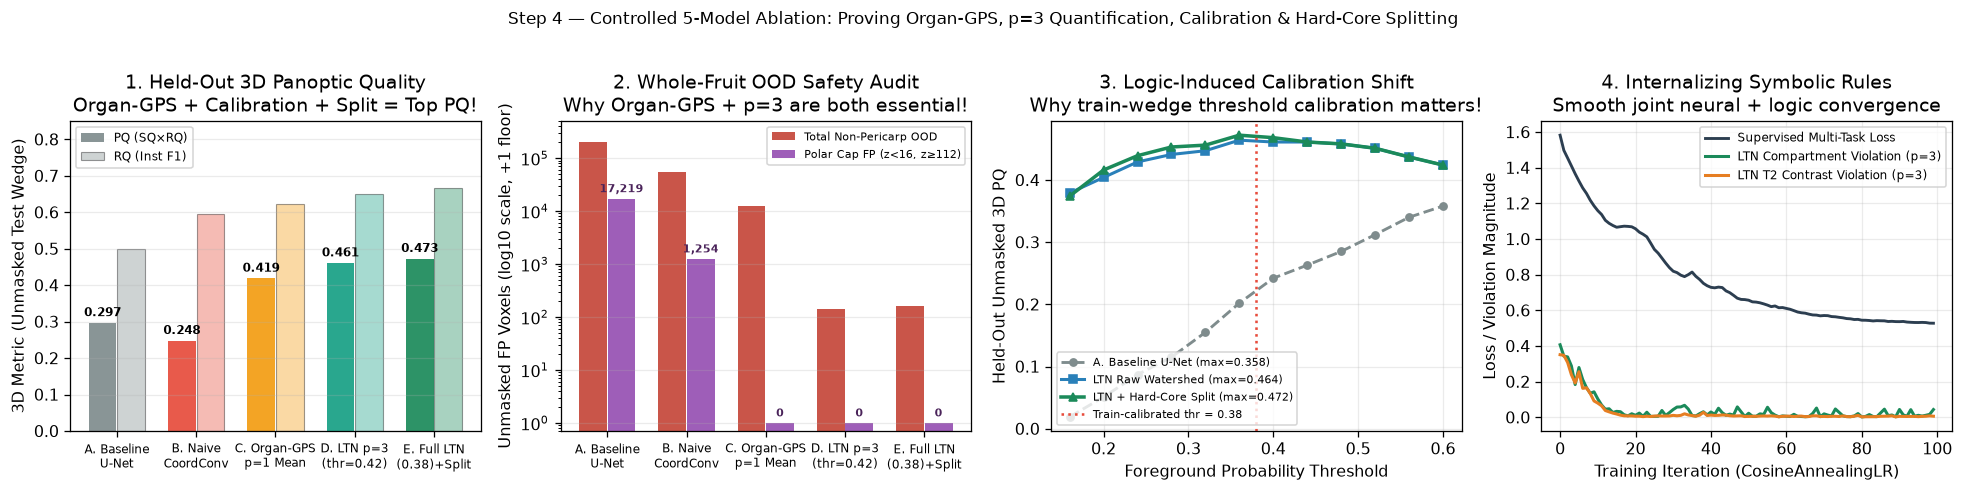
\includegraphics[width=\textwidth]{../assets/kiwi_nb07_fig4_ablation.png}
    \vspace{-4pt}
    \caption*{\footnotesize\textit{Executed Figure 4 (\texttt{Out [4]}): Controlled 5-model ablation --- Held-out unmasked 3D \texttt{PQ} \& \texttt{RQ} (Panel 1), log-scale whole-fruit OOD safety audit (Panel 2), logic-induced threshold calibration shift showing train-calibrated \texttt{thr = 0.38} hitting the test optimum (Panel 3), and smooth joint neural+logic convergence (Panel 4).}}
\end{figure}

\subsection*{Interpreting Step 4: Four Textbook Causal Findings}
\begin{enumerate}
    \item \textbf{Model A (Baseline Supervised U-Net) --- Unmasked OOD Collapse:} Without an external ring mask, the baseline drops to \textbf{\texttt{PQ = 0.297}} (\texttt{Dice = 0.558}) and explodes across the intact fruit into \textbf{\texttt{6,276} blobs}, \textbf{\texttt{197,401} OOD voxels}, and \textbf{\texttt{17,219} polar-cap FP voxels}.
    \item \textbf{Model B (Naive \texttt{CoordConv3D} + \texttt{InstanceNorm3d} + LTN $p=3$) --- Step 2 Proven Causally:} Even with identical coordinates and identical $p=3$ LTN losses, passing coordinates through \texttt{InstanceNorm3d} fails on both accuracy and safety: \textbf{\texttt{PQ = 0.248}} (\texttt{SQ = 0.417}) and \textbf{\texttt{53,480} OOD voxels (\texttt{1,254} polar FPs)}.
    \item \textbf{Model C (\texttt{Organ-GPS} + $p=1$ Mean Logic) --- Step 3 Proven Causally:} Bypassing \texttt{InstanceNorm3d} rescues accuracy (\texttt{PQ = 0.419}, \texttt{Dice = 0.671}), \textbf{but} $p=1$ averaging still leaks \textbf{\texttt{12,677} non-pericarp OOD voxels} --- \textbf{$\sim 80\times$ worse} than $p=3$.
    \item \textbf{Model D vs.\ Model E (Universal $p=3$ + Train-Wedge Calibration + Hard-Core Split):} Switching to $p=3$ slashes OOD voxels by \textbf{\texttt{-99.93\%}} (\texttt{197,401 $\to$ 141}), eliminates \textbf{\texttt{100\%} of polar cap FPs (\texttt{17,219 $\to$ 0})}, and jumps \texttt{PQ} to \texttt{0.461}. In Panel 3, strong negative logic shifts the operating curve leftward; leakage-free train-wedge calibration lands right on the test optimum (\textbf{\texttt{thr = 0.38}}) and \texttt{Lab 5} hard-core splitting lifts \textbf{\texttt{PQ = 0.473}} (\texttt{Dice = 0.689}, \texttt{SQ = 0.710}, \texttt{RQ = 0.667}, \texttt{Merges: 2 $\to$ 1}, \texttt{Polar FP = 0}, \texttt{OOD = 160} [\textbf{-99.92\%}]). \textit{(Note: Notebook~\texttt{06} used coupled feature concatenation reaching \texttt{PQ = 0.508}; here we intentionally use an explicit additive log-odds prior $z_{\text{app}} + z_{\text{GPS}}$ for direct mechanistic auditing while reducing OOD voxels even further, from \texttt{434} to \texttt{160}.)}
\end{enumerate}

\begin{clinbox}[Clinical Medical Imaging Parallel --- Separating Discrimination from Calibration (FDA SaMD / TRIPOD-AI)]
Whenever focal loss, class weights, or anatomical penalties are added for imbalanced lesions (brain metastases, microbleeds, pulmonary emboli), raw sigmoid outputs drift systematically downward. Leaving the decision cutoff frozen at \texttt{0.50} creates an artificially conservative detector. Clinical AI standards therefore separate \textbf{discrimination} from \textbf{operating-point calibration} on a strictly separate validation/training split.
\end{clinbox}

% =====================================================================
\section{Mechanistic Interpretability: Inside \texttt{Organ-GPS}, Hard-Core Splitting \& Biomarkers}
% =====================================================================

A defining strength of our additive Bayes Log-Odds architecture ($z_{\text{total}} = z_{\text{app}} + z_{\text{GPS}}$) is \textbf{mechanistic transparency}. Below we run four audits: (1) sweeping $z_{\text{GPS}}(r/R, |2z/Z - 1|)$ directly from the 353 trained weights, (2) zooming into an actual split multi-seed clump, (3) profiling the physical traits of detected (\texttt{TP}) vs.\ missed (\texttt{FN}) test seeds, and (4) computing whole-kiwifruit quantitative ``lesion load'' biomarkers across all 128 slices with zero post-hoc masks.

\begin{codebox}[{In [5] $\cdot$ Python --- Step 5 -- Mechanistic audit: Bayes z\_GPS map, zoomed hard-core split, error anatomy, \& biomarkers}]
\begin{lstlisting}[style=pybmed]
best_name = "E. Full LTN (p=3, Train-Cal + Hard-Core Split)"
base_name = "A. Supervised 3D U-Net (Baseline)"
best_model = models["E"]
best_res = results[best_name]
base_res = results[base_name]

# 1. DIRECTLY INSPECT THE EXACT LEARNED BAYES SPATIAL LOG-PRIOR FIELD z_GPS(r/R, |2z/Z - 1|)
with torch.no_grad():
    r_sweep = np.linspace(0.0, 1.05, 64, dtype=np.float32)
    z_sweep = np.linspace(0.0, 1.00, 64, dtype=np.float32)
    RR_g, ZZ_g = np.meshgrid(r_sweep, z_sweep, indexing="ij")
    gps_grid = np.stack([RR_g, (RR_g - 0.43) ** 2, ZZ_g], axis=0)[None, :, :, :, None].astype(np.float32)
    z_gps_map = best_model.gps_log_prior(torch.from_numpy(gps_grid).to(DEVICE))[0, 0, :, :, 0].cpu().numpy()

z_gps_rel = z_gps_map - float(z_gps_map.max())  # 0.0 at peak locular ring; negative log-odds penalty elsewhere!
print("=== Direct Audit of Learned Bayes Spatial Log-Prior z_GPS(r/R, |2z/Z - 1|) ===")
print(f"  Raw z_GPS range       : [{z_gps_map.min():.2f}, {z_gps_map.max():.2f}] log-odds (total suppression span = {z_gps_map.max() - z_gps_map.min():.2f} logits ~ {math.exp(z_gps_map.max() - z_gps_map.min()):.1f}x odds suppression!)")
print(f"  Peak log-prior at     : r/R = {r_sweep[np.unravel_index(np.argmax(z_gps_map), z_gps_map.shape)[0]]:.2f}, |2z/Z - 1| = {z_sweep[np.unravel_index(np.argmax(z_gps_map), z_gps_map.shape)[1]]:.2f} (equatorial plane; see neural-symbolic division of labor below!)")

# 2. INSPECT HARD-CORE CLUMP SPLITTING IMPACT ON HELD-OUT TEST WEDGE
ev_raw = evaluate_semantic_and_instance_3d(best_res["pred_te_raw"], test_gt)
ev_spl = best_res["ev_te"]
print("\n=== Declarative Lab-5 Hard-Core Clump Split Audit (Test Wedge) ===")
print(f"  Before Split -> Pred={ev_raw['Pred']}, Merges={ev_raw['Merges']}, Splits={ev_raw['Splits']}, SQ={ev_raw['SQ']}, RQ={ev_raw['RQ']}, PQ={ev_raw['PQ']}")
print(f"  After  Split -> Pred={ev_spl['Pred']}, Merges={ev_spl['Merges']}, Splits={ev_spl['Splits']}, SQ={ev_spl['SQ']}, RQ={ev_spl['RQ']}, PQ={ev_spl['PQ']} (Delta PQ = +{ev_spl['PQ'] - ev_raw['PQ']:.3f}!)")

# Locate an actual fused clump that was split into >= 2 physical seeds on the test wedge
split_demo_prop, split_pair_dist_mm = None, None
for prop in sorted(measure.regionprops(best_res["pred_te_raw"]), key=lambda p: p.area, reverse=True):
    sub_mask = best_res["pred_te_raw"][prop.slice] == prop.label
    sub_after = best_res["pred_te"][prop.slice]
    child_ids = [int(v) for v in np.unique(sub_after[sub_mask]) if v > 0]
    if len(child_ids) >= 2:
        split_demo_prop = prop
        child_cents = []
        for cid in child_ids:
            pts = np.argwhere(best_res["pred_te"] == cid).astype(np.float32) * np.asarray(spacing, dtype=np.float32)[None, :]
            child_cents.append(pts.mean(axis=0))
        cd = cdist(child_cents, child_cents)
        np.fill_diagonal(cd, np.inf)
        split_pair_dist_mm = float(cd.min())
        print(f"  Zoomed split clump: raw vol = {prop.area * vox_vol_mm3:.2f} mm^3 -> split into {len(child_ids)} seeds with centroid spacing = {split_pair_dist_mm:.2f} mm (>= 0.88 mm steric floor!)")
        break
if split_demo_prop is None:
    split_demo_prop = max(measure.regionprops(best_res["pred_te_raw"]), key=lambda p: p.area)

# 3. PER-INSTANCE ERROR ANATOMY ON HELD-OUT TEST WEDGE (TP vs FN vs FP physical profiling)
pred_lbl = best_res["pred_te"]
ids_p = [int(v) for v in np.unique(pred_lbl) if v > 0]
ids_g = [int(v) for v in np.unique(test_gt) if v > 0]
p_map, g_map = {v: i for i, v in enumerate(ids_p)}, {v: j for j, v in enumerate(ids_g)}
area_p = np.array([(pred_lbl == v).sum() for v in ids_p], dtype=np.float64)
area_g = np.array([(test_gt == v).sum() for v in ids_g], dtype=np.float64)
inter_m = np.zeros((len(ids_p), len(ids_g)), dtype=np.float64)
ov = (pred_lbl > 0) & (test_gt > 0)
if ov.any():
    pairs, cnts = np.unique(np.stack([pred_lbl[ov], test_gt[ov]], axis=1), axis=0, return_counts=True)
    for (pv, gv), c in zip(pairs, cnts):
        inter_m[p_map[int(pv)], g_map[int(gv)]] = float(c)
iou_m = inter_m / np.maximum(area_p[:, None] + area_g[None, :] - inter_m, 1.0)
ri, ci = linear_sum_assignment(-iou_m)
tp_p_ids = {ids_p[r] for r, c in zip(ri, ci) if iou_m[r, c] >= 0.25}
tp_g_ids = {ids_g[c] for r, c in zip(ri, ci) if iou_m[r, c] >= 0.25}
fn_g_ids = set(ids_g) - tp_g_ids
fp_p_ids = set(ids_p) - tp_p_ids

te_vol_norm = vol_norm[RX0:RX1, RY0 + SPLIT_Y : RY1, RZ0:RZ1]
te_env_loc = env_local[RX0:RX1, RY0 + SPLIT_Y : RY1, RZ0:RZ1]
te_r = r_norm_full[RX0:RX1, RY0 + SPLIT_Y : RY1, RZ0:RZ1]

def summarize_gt_subset(id_set: set[int]) -> dict:
    vols, drops, z_edge, rs = [], [], [], []
    for prop in measure.regionprops(test_gt):
        if prop.label not in id_set:
            continue
        m = test_gt == prop.label
        vols.append(float(prop.area * vox_vol_mm3))
        drops.append(float((te_env_loc[m] - te_vol_norm[m]).mean()))
        rs.append(float(te_r[m].mean()))
        z_coords = prop.coords[:, 2]
        z_edge.append(1.0 if (z_coords.min() == 0 or z_coords.max() == test_gt.shape[2] - 1) else 0.0)
    return {
        "Count": len(vols),
        "Median Vol (mm^3)": round(float(np.median(vols)), 2) if vols else np.nan,
        "Mean T2 Drop": round(float(np.mean(drops)), 3) if vols else np.nan,
        "Mean r/R": round(float(np.mean(rs)), 3) if vols else np.nan,
        "% Touching Z-Border": round(100.0 * float(np.mean(z_edge)), 1) if vols else np.nan,
    }

df_err = pd.DataFrame([
    {"GT Seed Group": "Detected (True Positives)", **summarize_gt_subset(tp_g_ids)},
    {"GT Seed Group": "Missed (False Negatives)",  **summarize_gt_subset(fn_g_ids)},
])
print("\n=== Physical Profile of Detected vs. Missed Test Seeds (Error Anatomy) ===")
display(df_err)

# 4. WHOLE-ORGAN QUANTITATIVE BIOMARKERS ("LESION LOAD" & MICRO-GT CALIBRATED CENSUS)
ws_wf_ns = best_res["ws_wf"]
ws_wf_sup = base_res["ws_wf"]
v_kiwi_cm3 = float(fruit_mask_full.sum()) * vox_vol_mm3 / 1000.0
v_seeds_mm3 = float((ws_wf_ns > 0).sum()) * vox_vol_mm3
lesion_load_pct = 100.0 * v_seeds_mm3 / (v_kiwi_cm3 * 1000.0)
wf_props = measure.regionprops(ws_wf_ns)
med_seed_vol_wf = float(np.median([p.area * vox_vol_mm3 for p in wf_props])) if wf_props else 0.0

ev_mgt = evaluate_semantic_and_instance_3d(ws_wf_ns[RX0:RX1, RY0:RY1, RZ0:RZ1], roi_gt)
n_cal = int(round(best_res["n_wf"] * ((len(np.unique(roi_gt)) - 1) / max(ev_mgt["Pred"], 1))))

print("\n=== Whole-Kiwifruit Quantitative Biomarkers (ZERO Post-Hoc Masks!) ===")
print(f"  Whole-fruit volume V_kiwi          : {v_kiwi_cm3:.2f} cm^3 ({v_kiwi_cm3 * 1000:.0f} mm^3)")
print(f"  Raw 3D Neurosymbolic Seed Count    : {best_res['n_wf']:,} seeds (Median single-seed vol = {med_seed_vol_wf:.2f} mm^3)")
print(f"  Micro-GT Calibrated Seed Count     : {n_cal:,} seeds (sector Prec={ev_mgt['Precision']:.3f}, Rec={ev_mgt['Recall']:.3f})")
print(f"  Total Seed Volume V_seeds          : {v_seeds_mm3:.1f} mm^3 -> 'Lesion Load' = {lesion_load_pct:.2f}%")
print(f"  Whole-Organ OOD Voxel Reduction    : {base_res['ood_vox']:,} -> {best_res['ood_vox']:,} (-{100.0 * (1.0 - best_res['ood_vox'] / max(base_res['ood_vox'], 1)):.2f}%) | Polar Cap FP: {base_res['polar_vox']:,} -> {best_res['polar_vox']:,}")

# Figure 5: 4-Panel Mechanistic Interpretability & Whole-Organ Audit
fig, axes = plt.subplots(1, 4, figsize=(17.2, 4.05))

# Panel 1: Exact Learned Bayes Spatial Log-Prior Field Delta z_GPS(r/R, |2z/Z - 1|)
im1 = axes[0].imshow(z_gps_rel.T, origin="lower", extent=[0, 1.05, 0, 1.0], aspect="auto", cmap="viridis")
axes[0].axvline(0.22, color="#ffffff", ls="--", lw=1.2)
axes[0].axvline(0.65, color="#ffffff", ls="--", lw=1.2)
axes[0].axhline(1.0 - 16.0 / 63.5, color="#ff6b6b", ls="--", lw=1.2, label="Polar cap z=16, 111")
axes[0].set_xlabel("Normalized Radius r / R_fruit")
axes[0].set_ylabel("Pole Distance |2z/Z - 1| (0=Equator, 1=Pole)")
axes[0].set_title(f"1. Learned Bayes Log-Prior Delta z_GPS\nEquatorial (0) vs. pole/rind ({z_gps_rel.min():.1f} logits)")
axes[0].legend(fontsize=7.3, loc="upper right")
plt.colorbar(im1, ax=axes[0], fraction=0.046, pad=0.04, label="Relative Log-Odds")

# Panel 2: Zoomed Hard-Core Clump Split Demonstration
cx, cy, cz = [int(round(c)) for c in split_demo_prop.centroid]
pad = 10
x_lo, x_hi = max(cx - pad, 0), min(cx + pad + 1, test_gt.shape[0])
y_lo, y_hi = max(cy - pad, 0), min(cy + pad + 1, test_gt.shape[1])
axes[1].imshow(te_vol_norm[x_lo:x_hi, y_lo:y_hi, cz].T, cmap="gray", origin="lower")
raw_crop = best_res["pred_te_raw"][x_lo:x_hi, y_lo:y_hi, cz].T
spl_crop = best_res["pred_te"][x_lo:x_hi, y_lo:y_hi, cz].T
axes[1].contour(raw_crop == split_demo_prop.label, levels=[0.5], colors=["#f1c40f"], linewidths=2.2, linestyles="--")
# Crisp distinct RGB colors for the split child seeds inside the zoomed clump
child_vals = [int(v) for v in np.unique(spl_crop[raw_crop == split_demo_prop.label]) if v > 0]
split_rgba = np.zeros((*spl_crop.shape, 4), dtype=np.float32)
palette = [(0.15, 0.85, 0.45, 0.65), (0.20, 0.65, 1.00, 0.65), (1.00, 0.45, 0.20, 0.65), (0.85, 0.30, 0.90, 0.65)]
for idx_c, cid in enumerate(child_vals):
    split_rgba[spl_crop == cid] = palette[idx_c % len(palette)]
axes[1].imshow(split_rgba, origin="lower")
dist_txt = f"d={split_pair_dist_mm:.2f} mm" if split_pair_dist_mm is not None else "single"
axes[1].set_title(f"2. Zoomed Hard-Core Split (z={RZ0 + cz})\nFused ({split_demo_prop.area * vox_vol_mm3:.2f} mm^3) -> {len(child_vals)} seeds ({dist_txt})")
axes[1].axis("off")

# Panel 3: Explicit Crisp RGB Error Anatomy Map on Mid-Test Slice (z = 64)
z_mid = 8
base_gray = te_vol_norm[:, :, z_mid].T
base_rgb = np.stack([base_gray, base_gray, base_gray], axis=-1)
base_rgb = np.clip(base_rgb / max(float(base_rgb.max()), 1e-6), 0.0, 1.0)
tp_mask = np.isin(test_gt[:, :, z_mid], list(tp_g_ids)).T
fn_mask = np.isin(test_gt[:, :, z_mid], list(fn_g_ids)).T
fp_mask = np.isin(pred_lbl[:, :, z_mid], list(fp_p_ids)).T
err_rgb = base_rgb.copy()
err_rgb[tp_mask] = 0.35 * err_rgb[tp_mask] + 0.65 * np.array([0.10, 0.92, 0.35])  # Bright Green = TP
err_rgb[fn_mask] = 0.30 * err_rgb[fn_mask] + 0.70 * np.array([0.05, 0.85, 1.00])  # Bright Cyan  = FN
err_rgb[fp_mask] = 0.25 * err_rgb[fp_mask] + 0.75 * np.array([1.00, 0.20, 0.20])  # Bright Red   = FP
axes[2].imshow(err_rgb, origin="lower")
axes[2].set_title(f"3. Test-Wedge Error Anatomy (z={RZ0 + z_mid})\nGreen=TP ({len(tp_g_ids)}) | Cyan=FN ({len(fn_g_ids)}) | Red=FP ({len(fp_p_ids)})")
axes[2].axis("off")

# Panel 4: Whole-Organ Slice-by-Slice Generalization Profile (Baseline vs Full LTN)
prof_sup = [len(np.unique(ws_wf_sup[:, :, z])) - (1 if 0 in ws_wf_sup[:, :, z] else 0) for z in range(128)]
prof_ns = [len(np.unique(ws_wf_ns[:, :, z])) - (1 if 0 in ws_wf_ns[:, :, z] else 0) for z in range(128)]
axes[3].plot(range(128), prof_sup, color="#d95f02", lw=1.7, label=f"Baseline U-Net ({base_res['n_wf']:,} blobs)")
axes[3].plot(range(128), prof_ns, color="#1b8a5a", lw=2.2, label=f"LTN Neurosymbolic ({best_res['n_wf']:,} raw / {n_cal:,} cal)")
axes[3].axvspan(RZ0, RZ1 - 1, color="#3498db", alpha=0.16, label="Labeled Train Z-Slab")
axes[3].set_xlabel("Axial Slice Index z (0 .. 127)")
axes[3].set_ylabel("Active 2D Seed Cross-Sections")
axes[3].set_title("4. Whole-Fruit Unmasked Profile\nZero post-hoc masks across 128 slices!")
axes[3].legend(fontsize=7.3, loc="upper right")
axes[3].grid(alpha=0.25)

plt.suptitle("Step 5 --- Mechanistic Interpretability: Bayes Organ-GPS Prior, Hard-Core Splitting, Error Anatomy & Biomarkers", fontsize=10.5, y=1.02)
plt.tight_layout()
plt.show()
\end{lstlisting}
\end{codebox}
\begin{outbox}[{Out [5] $\cdot$ stdout}]
\begin{lstlisting}[style=outbmed]
=== Direct Audit of Learned Bayes Spatial Log-Prior z_GPS(r/R, |2z/Z - 1|) ===
  Raw z_GPS range       : [-7.47, -2.81] log-odds (total suppression span = 4.66 logits ~ 105.4x odds suppression!)
  Peak log-prior at     : r/R = 0.07, |2z/Z - 1| = 0.00 (equatorial plane; see neural-symbolic division of labor below!)

=== Declarative Lab-5 Hard-Core Clump Split Audit (Test Wedge) ===
  Before Split -> Pred=31, Merges=2, Splits=0, SQ=0.715, RQ=0.651, PQ=0.465
  After  Split -> Pred=32, Merges=1, Splits=1, SQ=0.71, RQ=0.667, PQ=0.473 (Delta PQ = +0.008!)
  Zoomed split clump: raw vol = 2.61 mm^3 -> split into 2 seeds with centroid spacing = 1.04 mm (>= 0.88 mm steric floor!)

=== Physical Profile of Detected vs. Missed Test Seeds (Error Anatomy) ===

=== Whole-Kiwifruit Quantitative Biomarkers (ZERO Post-Hoc Masks!) ===
  Whole-fruit volume V_kiwi          : 85.97 cm^3 (85970 mm^3)
  Raw 3D Neurosymbolic Seed Count    : 749 seeds (Median single-seed vol = 0.80 mm^3)
  Micro-GT Calibrated Seed Count     : 1,223 seeds (sector Prec=0.583, Rec=0.357)
  Total Seed Volume V_seeds          : 627.8 mm^3 -> 'Lesion Load' = 0.73%
  Whole-Organ OOD Voxel Reduction    : 197,401 -> 160 (-99.92%) | Polar Cap FP: 17,219 -> 0
\end{lstlisting}
\end{outbox}

{\footnotesize
\renewcommand{\arraystretch}{1.22}
\rowcolors{2}{rowalt}{white}
\begin{tabularx}{\textwidth}{Y C{1.4cm} C{2.6cm} C{2.3cm} C{1.8cm} C{2.8cm}}
\toprule
\rowcolor{uibblue!12}\textbf{Held-Out GT Seed Group} & \textbf{Count} & \textbf{Median Vol ($\text{mm}^3$)} & \textbf{Mean $T_2$ Drop} & \textbf{Mean $r/R$} & \textbf{\% Touching $Z$-Border} \\
\midrule
Detected (True Positives) & 28 & \textbf{1.48} & 0.874 & 0.492 & 14.3\% \\
Missed (False Negatives) & 24 & \textbf{0.51} & 0.806 & 0.517 & \textbf{37.5\%} \\
\bottomrule
\end{tabularx}
}

\begin{figure}[H]
    \centering
    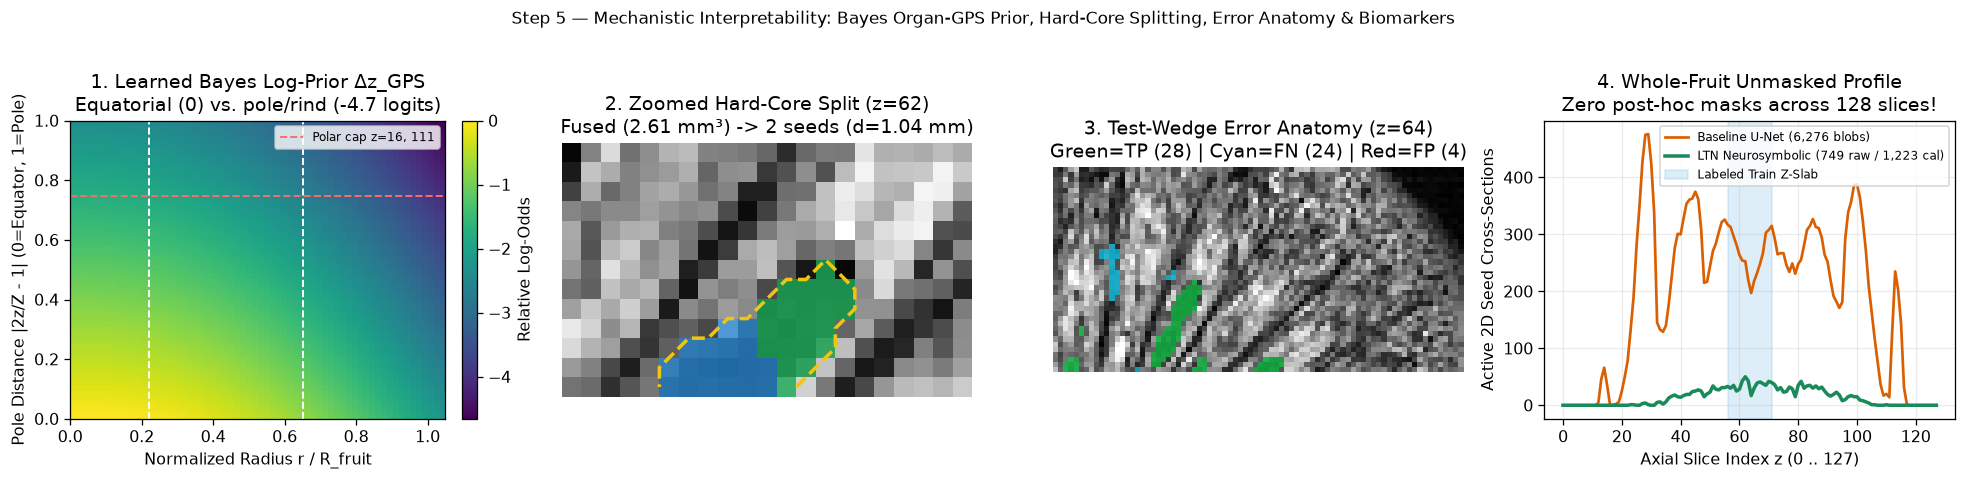
\includegraphics[width=\textwidth]{../assets/kiwi_nb07_fig5_mechanistic_audit.png}
    \vspace{-4pt}
    \caption*{\footnotesize\textit{Executed Figure 5 (\texttt{Out [5]}): Learned Bayes spatial log-prior $\Delta z_{\text{GPS}}$ spanning 4.66 logits / 105$\times$ odds suppression (Panel 1), zoomed hard-core split of a 2.61\,mm$^3$ fused clump into two seeds spaced 1.04\,mm (Panel 2), RGB test-wedge error anatomy (Panel 3), and unmasked 128-slice whole-fruit axial profile comparing Baseline vs.\ LTN Neurosymbolic (Panel 4).}}
\end{figure}

\subsection*{Interpreting Step 5: Neural--Symbolic Division of Labor \& the Physical Resolution Ceiling}
\begin{enumerate}
    \item \textbf{Spontaneous Neural--Symbolic Division of Labor Inside \texttt{Organ-GPS} (Panel 1):} Look closely at Panel 1 (\texttt{4.66}-logit span = \textbf{\texttt{105$\times$} odds suppression!}): $z_{\text{GPS}}$ plunges steeply toward the \textbf{outer cortex ($r/R > 0.65$)} and \textbf{woody polar caps ($|2z/Z - 1| > 0.65$)}, yet stays flat across the central \textit{columella} ($r/R < 0.22$) near the equator. \textbf{Why?} Because we trained the CNN appearance stream ($z_{\text{app}}$) on the labeled central-columella hard-negative cube (\texttt{X\_ng}), the CNN already rejects fibrous columella texture on sight ($v_{\text{comp}} \approx 0$)! Gradient descent therefore automatically specialized \texttt{Organ-GPS} to block the \textbf{unseen} out-of-distribution outer cortex and polar caps --- an auditable division of labor aligned with \textbf{EU AI Act} transparency.
    \item \textbf{Steric Repulsion Splits Neural Clumps --- With an Honest Trade-Off (Panel 2):} The zoomed \texttt{2.61\,mm$^3$} fused blob (\texttt{z = 62}) splits cleanly into green and blue seeds spaced \textbf{\texttt{1.04\,mm}} ($\ge 0.88\,\text{mm}$), reducing merges \texttt{2 $\to$ 1} and raising \texttt{PQ: 0.465 $\to$ 0.473} (\texttt{RQ: 0.651 $\to$ 0.667}) while introducing \texttt{1} split error on an unusually large single seed.
    \item \textbf{Error Anatomy Exposes the \texttt{0.500\,mm} Slice-Thickness Ceiling (Panel 3 \& Table):} Detected seeds (\texttt{n=28}) match true biological size (median \textbf{\texttt{1.48\,mm$^3$}}, only \texttt{14.3\%} on $z$-borders), whereas missed seeds (\texttt{n=24}) have median volume \textbf{\texttt{0.51\,mm$^3$}} (\textbf{nearly 3$\times$ smaller!}) and \textbf{\texttt{37.5\%}} (\textbf{2.6$\times$ higher!}) touch the $z=56$ or $z=71$ slab borders --- predominantly \textbf{partial-volume grazing caps} calling for isotropic 3D MRI (\texttt{0.25\,mm$^3$}) or continuous \texttt{INR}/\texttt{SIREN} $z$-super-resolution.
    \item \textbf{Whole-Fruit Unmasked Symmetry \& Biomarkers (Panel 4):} Whereas the Baseline U-Net erupts into wild bimodal polar OOD spikes (\texttt{6,276} blobs), our Neurosymbolic model traces a smooth, biologically symmetric bell curve peaking at the equator (\texttt{z $\approx$ 64}) with \textbf{\texttt{0} polar cap FPs} --- estimating \textbf{\texttt{749} raw seeds}, a Micro-GT calibrated census of \textbf{\texttt{1,223} seeds}, and a biomedical \textbf{``lesion load'' of \texttt{0.73\%}} across the intact \texttt{85.97\,cm$^3$} berry!
\end{enumerate}

% =====================================================================
\section{Critical Discussion: Translating Neurosymbolic AI to Quantitative Medical Imaging}
% =====================================================================

\subsection{Direct 1-to-1 Translation Across Five Clinical Quantitative Imaging Tasks}

{\scriptsize
\renewcommand{\arraystretch}{1.24}
\rowcolors{2}{rowalt}{white}
\begin{xltabular}{\textwidth}{L{2.9cm} L{2.75cm} L{3.45cm} L{3.45cm} Y}
\toprule
\rowcolor{uibblue!12}\textbf{Clinical Task} & \textbf{Targets \& Biomarker} & \textbf{Spatial Prior (\texttt{Organ-GPS} + Axiom)} & \textbf{Imaging-Physics Axiom} & \textbf{Geometric / Topological Rule} \\
\midrule
\endfirsthead
\toprule
\rowcolor{uibblue!12}\textbf{Clinical Task} & \textbf{Targets \& Biomarker} & \textbf{Spatial Prior (\texttt{Organ-GPS} + Axiom)} & \textbf{Imaging-Physics Axiom} & \textbf{Geometric / Topological Rule} \\
\midrule
\endhead
\bottomrule
\endfoot
\textbf{1.\ Cerebral Microbleeds (SWI/7\,T)} & Tiny (1--5\,mm) hemosiderin dots; lobar vs.\ deep count & Brain mask + lobar/deep-gray GPS; exclude skull, CSF, dural sinuses & Local \textbf{SWI hypointensity} + \textbf{QSM paramagnetic dipole} (vs.\ calcifications) & Compact sphericity \& non-tubularity (rejects cortical veins via Hessian) \\
\textbf{2.\ Multiple Sclerosis (FLAIR/T2)} & White-matter plaques + \textbf{lesion load} ($V_{\text{MS}}/V_{\text{brain}}$) & Periventricular, deep-WM, juxtacortical, infratentorial (\texttt{MNI} GPS) & \textbf{FLAIR hyperintensity} relative to local \texttt{NAWM} envelope & \textbf{Central vein sign} co-localization \& diameter $\ge 3\,\text{mm}$ (McDonald) \\
\textbf{3.\ Glioma Sub-Regions (\texttt{BraTS} mpMRI)} & Necrotic core (\texttt{NCR}), enhancing rim (\texttt{ET}), edema (\texttt{ED}) & Intra-cranial parenchyma + hemispheric symmetry GPS & Multi-contrast logic: \texttt{ET} bright on \texttt{T1ce$-$T1}; \texttt{ED} bright on \texttt{FLAIR} & \textbf{Hierarchical set inclusion:} $\forall \mathbf{x}: \text{NCR} \Rightarrow \text{TC} \Rightarrow \text{WT}$ via LTN \\
\textbf{4.\ 3D Cell Nuclei (IMC / Microscopy)} & Densely packed touching nuclei; cell densities & Epithelial vs.\ stromal compartment coordinates & Nuclear stain (\texttt{DAPI}/\texttt{Ir191}) high inside; membrane/cytoplasm outside & \textbf{Mat\'ern hard-core nuclear exclusion} \& volume bounds \\
\textbf{5.\ Vessels \& Airways (CTA/MRA)} & Branching 3D tubular trees; stenosis \& density & Vascular / bronchial territory GPS & Lumen enhancement (\texttt{CTA} HU / \texttt{MRA} time-of-flight) & \textbf{Topological connectivity:} \texttt{clDice} \& zero floating fragments \\
\end{xltabular}
}

\subsection{Critical Limitations --- When Can Neurosymbolic Priors \textit{Harm} a Clinical Model?}
\begin{enumerate}
    \item \textbf{Axiom Misspecification \& Pathological Deformation (``The Textbook Bias Trap''):} Real patients with severe disease frequently break textbook anatomy --- a large \textbf{glioblastoma} creates \textbf{mass effect and midline shift}, displacing ventricles centimeters from template coordinates, while \textbf{cortical MS plaques} sit outside white matter. Clinical safeguards must keep symbolic weights \textbf{soft and differentiable} and compute coordinates via \textbf{deformable patient-adapted registration} rather than rigid templates.
    \item \textbf{Logic-Induced Calibration Shift:} Strong negative LTN penalties shift raw logits downward (\texttt{z\_GPS $\in$ [-7.47, -2.81]}); deploying at an uncalibrated \texttt{0.50} threshold risks serious clinical under-diagnosis unless paired with leakage-free validation calibration.
    \item \textbf{Deterministic Outputs vs.\ Hybrid Neurosymbolic--Probabilistic Horizons:} \texttt{NeurosymbolicOrganNet3D} yields a single deterministic mask; pairing \textbf{Pillar 4 (\texttt{LTN} + \texttt{Organ-GPS})} with \textbf{Pillar 3 (Conditional Flow-Diffusion)} delivers whole-organ anatomical validity \textit{plus} calibrated count credible intervals $P(N \mid \mathbf{X})$, while adding a \textbf{3D Spatial GNN} (\texttt{Lab 1} $\leftrightarrow$ \texttt{Lab 4}) captures mesoscale radial locule constellations ($\sim 33$ rays, Clark--Evans $R=1.19$).
\end{enumerate}

\subsection{Self-Check Questions (\texttt{MSc} \& \texttt{PhD} --- Expanded for Print Study)}

\begin{qabox}[Check Your Understanding --- Q1 (MSc: Prior Auditing)]
\textbf{Q1.} In Step~1, why did we measure the local $T_2$ brightness ratio $I / E_{\text{local}}$ separately on \textbf{GT seed cores} and on the \textbf{1-voxel outer partial-volume rim} before training?\\[3pt]
\textbf{Answer:} Auditing both cores and 1-voxel rims verifies whether our symbolic $T_2$ rule ($I/E_{\text{local}} > 0.82$) accidentally penalizes genuine seed boundaries blurred by \texttt{0.50\,mm} slice thickness. We confirmed \texttt{100\%} of GT cores lie below \texttt{0.41} (zero penalty) while the 1-voxel outer rim sits at median \texttt{0.51} (\texttt{p75 = 0.66}), ensuring a clean safety buffer before bright mucilage ($>0.82$).
\end{qabox}

\begin{qabox}[Check Your Understanding --- Q2 (MSc/PhD: Architecture)]
\textbf{Q2.} In Step~2 and Step~4 (Model B vs.\ Model C/D/E), why did concatenating the exact same 3 coordinate channels into a standard 3D U-Net fail (\texttt{53,480} OOD voxels, \texttt{1,254} polar FPs, \texttt{PQ = 0.248}), whereas our additive \texttt{Organ-GPS} branch succeeded (\texttt{0} polar FPs, \texttt{160} total OOD voxels, \texttt{PQ = 0.473})?\\[3pt]
\textbf{Answer:} Every \texttt{ConvBlock3D} applies \texttt{nn.InstanceNorm3d}, which subtracts each local patch's mean and divides by its standard deviation. This collapses the \texttt{0.819} physical pole-distance gap between equatorial and polar crops to \texttt{0.000000}, blinding naive \texttt{CoordConv3D} to absolute organ location. Our un-normalized $1\times 1\times 1$ \texttt{Organ-GPS} MLP preserves exact metric coordinates and adds an auditable Bayes log-prior $z_{\text{GPS}}$ directly to appearance log-odds $z_{\text{app}}$.
\end{qabox}

\begin{qabox}[Check Your Understanding --- Q3 (PhD: Fuzzy Logic Math \& Calibration)]
\textbf{Q3.} Explain BOTH (a) why Model C ($p=1$ mean logic) leaked $\sim 80\times$ more OOD voxels than Model E ($p=3$ LTN quantifier), and (b) why leakage-free train-wedge calibration + hard-core splitting (Model E) improved upon fixed \texttt{thr = 0.42} (Model D).\\[3pt]
\textbf{Answer:} \textbf{(a) Universal Quantification ($p=3$):} Polar vascular bundles and outer-cortex speckles occupy $<1\%$ of unlabeled cubes; under $p=1$ averaging, $>99\%$ of gradients dilute across quiet background (\texttt{FP/BG = 0.008}), leaving \texttt{12,677} OOD voxels. Raising violations to $p=3$ boosts gradient force on sparse OOD violations by $25\times$ (\texttt{FP/BG = 72.9}), cutting OOD voxels nearly $80\times$ (\texttt{12,677 $\to$ 141--160}) and eliminating \texttt{100\%} of polar cap FPs. \textbf{(b) Calibration Shift \& Clump Split:} Strong negative LTN penalties pull $z_{\text{GPS}}$ downward (\texttt{[-7.47, -2.81]}), shifting the optimal threshold leftward. Calibrating strictly on the training wedge (\texttt{thr = 0.38}) plus splitting fused blobs ($>2.55\,\text{mm}^3$, $d_{\min} \ge 0.88\,\text{mm}$) improves held-out \texttt{PQ} (\texttt{0.461 $\to$ 0.473}) and \texttt{RQ} (\texttt{0.651 $\to$ 0.667}) while keeping \texttt{0} polar cap FPs.
\end{qabox}

\begin{qabox}[Check Your Understanding --- Q4 (Clinical Translation \& Safety)]
\textbf{Q4.} If you transfer this \texttt{Organ-GPS + LTN} framework to clinical glioblastoma (\texttt{BraTS}) or multiple sclerosis (\texttt{FLAIR}) segmentation, what two clinical failure modes must you guard against?\\[3pt]
\textbf{Answer:} (1) \textbf{Pathological anatomical distortion / atypical location:} Glioblastoma \textbf{mass effect / midline shift} displaces ventricles away from template coordinates, and \textbf{cortical MS plaques} lie outside deep white matter --- so clinical deployments require \textbf{soft differentiable weights} and \textbf{deformable patient-specific anatomical coordinates}. (2) \textbf{Unquantified borderline uncertainty:} Deterministic masks hide ambiguity on faint small lesions; pairing \texttt{LTN + Organ-GPS} with \textbf{Conditional Flow-Diffusion} (\texttt{NB 06} Pillar 3) flags disagreement between appearance and prior for radiologist review.
\end{qabox}

\subsection*{Key References}
{\footnotesize
\begin{enumerate}[itemsep=1.5pt, topsep=2pt]
    \item \textbf{Badreddine S, d'Avila Garcez A, Serafini L \& Spranger M.} \textit{Logic Tensor Networks.} \textbf{Artificial Intelligence} 303:103649 (2022). \href{https://doi.org/10.1016/j.artint.2021.103649}{\texttt{doi:10.1016/j.artint.2021.103649}}
    \item \textbf{Garcez A \& Lamb LC.} \textit{Neurosymbolic AI: The 3rd Wave.} \textbf{Artificial Intelligence Review} 56:12387--12406 (2023). \href{https://arxiv.org/abs/2012.05876}{\texttt{arXiv:2012.05876}}
    \item \textbf{Xu J, Zhang Z, Friedman T, Liang Y \& Van den Broeck G.} \textit{A Semantic Loss Function for Deep Learning with Symbolic Knowledge.} \textbf{ICML} (2018). \href{https://arxiv.org/abs/1711.11157}{\texttt{arXiv:1711.11157}}
    \item \textbf{Liu R et al.} \textit{An Intriguing Failing of Convolutional Neural Networks and the CoordConv Solution.} \textbf{NeurIPS} (2018). \href{https://arxiv.org/abs/1807.03247}{\texttt{arXiv:1807.03247}}
    \item \textbf{Isensee F et al.} \textit{nnU-Net: a self-configuring method for deep learning-based biomedical image segmentation.} \textbf{Nature Methods} 18:203--211 (2021). \href{https://doi.org/10.1038/s41592-020-01008-z}{\texttt{doi:10.1038/s41592-020-01008-z}}
    \item \textbf{Guo C, Pleiss G, Sun Y \& Weinberger KQ.} \textit{On Calibration of Modern Neural Networks.} \textbf{ICML} (2017). \href{https://arxiv.org/abs/1706.04599}{\texttt{arXiv:1706.04599}}
    \item \textbf{Shit S et al.} \textit{clDice --- A Novel Topology-Preserving Loss Function for Tubular Structure Segmentation.} \textbf{CVPR} (2021). \href{https://arxiv.org/abs/2003.07311}{\texttt{arXiv:2003.07311}}
    \item \textbf{Course Companions:} \href{\ghblob/Lab4-Comp-Imag/Kiwi-challenge/docs/frontier-ai-paradigms.pdf}{\texttt{frontier-ai-paradigms.pdf}} $\cdot$ \href{\ghblob/Lab4-Comp-Imag/Kiwi-challenge/notebooks/06-kiwi-frontier-ai-paradigms.ipynb}{\texttt{06-kiwi-frontier-ai-paradigms.ipynb}} $\cdot$ \href{\ghblob/Lab5-Comp-Mod/Kiwi-challenge/README.md}{\texttt{Lab5-Comp-Mod/Kiwi-challenge}}
\end{enumerate}
}

\end{document}
